\begin{center}
\vfill
    \chapter{Meccanica classica}
    \label{blx:Meccanica-Classica\therefsection}
\vfill

\minitoc
\newpage
\end{center}
\justify

\section{Cenni di meccanica classica}\label{cenni-di-meccanica-classica}

La \textbf{meccanica} è la branca della fisica che studia il moto dei corpi materiali \cite{landau1994meccanica}. In base alle caratteristiche fisiche della materia considerata, sono state sviluppate diverse teorie meccaniche, suddivise principalmente in:
\begin{itemize}
    \item \textbf{Meccanica classica}: descrive sistemi di dimensioni macroscopiche che si muovono a velocità molto inferiori rispetto a quella della luce;
    \item \textbf{Meccanica statistica}: applicabile a sistemi costituiti da un numero elevato di particelle, delle quali si analizzano le proprietà medie;
    \item \textbf{Meccanica relativistica}: tratta sistemi non quantistici che si muovono a velocità prossime a quella della luce;
    \item \textbf{Meccanica quantistica}: si occupa di sistemi su scala atomica e subatomica, dove gli effetti quantistici risultano predominanti.
\end{itemize}

\section{Meccanica newtoniana}\label{meccanica-newtoniana}
La \textbf{meccanica classica} si fonda sulla descrizione dei fenomeni fisici secondo l'approccio introdotto da Newton nel XVII secolo. Essa interpreta il moto della natura in termini di forze $\vec{F}$ e accelerazioni $\vec{a}$. Il punto di vista \textbf{newtoniano} si basa sull'equazione fondamentale del moto, valida nell'ipotesi in cui la massa è costante nel tempo:

\[
\vec{F} = m \vec{a}
\]

dove \(m\) è la massa della particella (assunta costante) e \(\vec{a}\) è la sua accelerazione. L'accelerazione è definita come la derivata della velocità rispetto al tempo:

\[
\vec{a} = \dfrac{d\vec{v}}{dt}
\]

Si definisce la \textbf{quantità di moto} (o \textbf{momento lineare}) \(\vec{p}\) come il prodotto tra la massa e la velocità della particella:

\[
\vec{p} = m\vec{v}
\]

Il vettore \(\vec{p}\) ha la stessa direzione e verso del vettore velocità \(\vec{v}\). L'equazione fondamentale della meccanica può essere riscritta in termini di quantità di moto:

\[
\vec{F} = m\vec{a} = m\dfrac{d\vec{v}}{dt} = \dfrac{d}{dt}(m\vec{v}) = \dfrac{d\vec{p}}{dt}
\]

Questa relazione rappresenta la forma più generale della Seconda Legge di Newton. Essa è valida anche nel caso in cui la massa $m$ non sia costante nel tempo (ad esempio, per un razzo che espelle propellente), mentre la forma $\vec{F} = m\vec{a}$ è valida solo quando la massa è costante.

L'equazione può essere estesa a un sistema di \(n\) particelle, con masse \(\{ m_{1},m_{2},\ldots,m_{n}\}\) e forze \(\{{\vec{f}}_{1},{\vec{f}}_{2},\ldots,{\vec{f}}_{n}\}\), ottenendo:

\[
{\vec{F}}_{\text{tot}} = \sum_{k = 1}^{n}{\vec{f}}_{k} = \sum_{k = 1}^{n}\dfrac{d{\vec{p}}_{k}}{dt} = \dfrac{d\vec{P}}{dt}
\]

Questa espressione rappresenta il \textbf{Teorema della quantità di moto} (o \textbf{Teorema della dinamica}) per i sistemi di particelle. Poiché la somma di tutte le forze interne ($\vec{F}_{\text{int}}$) è nulla per il Terzo Principio della Dinamica (Principio di azione e reazione), la forza totale ($\vec{F}_{\text{tot}}$) coincide con la risultante delle sole forze esterne ($\vec{F}_{\text{est}}$). Il teorema si scrive quindi:

\[
{\vec{F}}_{\text{est}} = \dfrac{d\vec{P}}{dt} \quad \text{con } \vec{P} = \sum_{k=1}^n \vec{p}_k
\]

\begin{figure}[H]
    \centering
    \resizebox{0.45\textwidth}{!}{%
    \begin{tikzpicture}[
        particle/.style={circle, draw, fill=blue!20, minimum size=10pt, inner sep=0pt},
        velocity/.style={-Latex, thick, red},
        axis/.style={-Latex, thick},
        origin/.style={circle, fill=black, inner sep=1.5pt},
        scale=1.0
    ]

    % Sistema di riferimento tridimensionale
    \coordinate (O) at (-1.5,-1.2);
    \node[origin, label={[xshift=3pt, yshift=-4pt]below left:{$O$}}] at (O) {}; % origine evidenziata
    \draw[axis] (O) -- ++(7,0) node[right] {$x$};
    \draw[axis] (O) -- ++(0,5) node[above] {$y$};
    \draw[axis] (O) -- ++(-1.8,-1.2) node[below left] {$z$};

    % Particelle
    \node[particle, label=left:{$m_1$}] (m1) at (0,0) {};
    \node[particle, label=below:{$m_2$}] (m2) at (2,0.5) {};
    \node[particle, label=right:{$m_3$}] (m3) at (4,0) {};
    \node[particle, label=above:{$m_4$}] (m4) at (1.5,2) {};
    \node[particle, label=above:{$m_5$}] (m5) at (3.5,1.8) {};

    % Vettori velocità
    \draw[velocity] (m1) -- ++(0.8,0.3) node[above ] {$\vec{v}_1$};
    \draw[velocity] (m2) -- ++(0.4,0.7) node[above ] {$\vec{v}_2$};
    \draw[velocity] (m3) -- ++(-0.7,0.2) node[above ] {$\vec{v}_3$};
    \draw[velocity] (m4) -- ++(0.3,-0.6) node[below ] {$\vec{v}_4$};
    \draw[velocity] (m5) -- ++(-0.5,-0.4) node[below ] {$\vec{v}_5$};

    % Particella generica m_i (spostata in alto a destra per visibilità)
    \node[particle, label=above right:{$m_i$}] (mi) at (4.8,2.4) {};
    % Vettore velocità ruotato per evitare sovrapposizione
    \draw[velocity] (mi) -- ++(-0.6,0.5) node[above left] {$\vec{v}_i$};

    \end{tikzpicture}

    }
    \caption{Sistema di particelle in un sistema di riferimento tridimensionale}
    \label{fig:1_sistPart}
\end{figure}


Per una particella soggetta a una forza \(\vec{F}\), si definisce \textbf{momento torcente} (o \textbf{momento della forza}) \(\vec{N}\) (talvolta indicato anche con \(\vec{\tau}\)):

\[
\vec{N} = \vec{r} \times \vec{F}
\]

dove \(\vec{r}\) è il vettore posizione della particella rispetto a un polo (origine del sistema di riferimento).

\begin{figure}[H]
    \centering
    \resizebox{0.44\textwidth}{!}{%
    \begin{tikzpicture}[scale=1.2]
    % Coordinate
    \coordinate (O) at (0,0);
    \coordinate (A) at (2,0);
    \coordinate (B) at (3,1);

    % Vettori
    \fill (O) circle (1pt);
    \node[left] at (O) {$O$};
    \draw[->, thick] (O) -- (A) node[midway, below] {$\vec{r}$};
    \draw[->, thick] (A) -- (B) node[midway, above] {$\vec{F}$};

    % Disegno dell'angolo tra i due vettori
    \draw (A) -- ++(-0.5,0) coordinate (aux); % punto ausiliario per l'arco
    \pic [draw, "$\theta$", angle radius=0.4cm] {angle = B--A--O};

\end{tikzpicture}

    }
    \caption{Definizione del momento torcente rispetto a un punto fisso}
    \label{fig:1_momTorc}
\end{figure}


Analogamente, si definisce \textbf{momento angolare} (o \textbf{quantità di moto angolare}) \(\vec{L}\):

\[
\vec{L} = \vec{r} \times \vec{p}
\]

\begin{figure}[H]
    \centering
    \resizebox{0.8\textwidth}{!}{%
    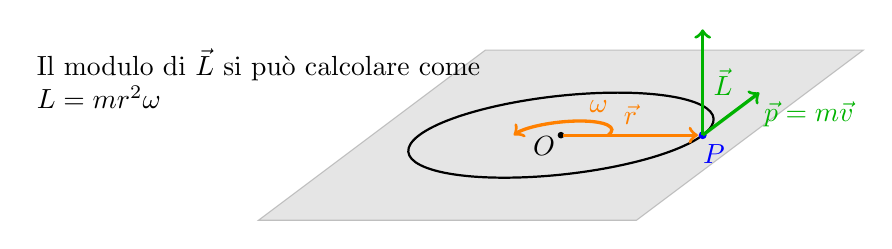
\begin{tikzpicture}[scale=1.2, x={(1cm,0cm)}, y={(0.4cm,0.3cm)}, z={(0cm,0.7cm)}]

    % Piano grigio con ombra
    \fill[gray!20] (-2,-3,0) -- (2,-3,0) -- (2,3,0) -- (-2,3,0) -- cycle;
    \draw[gray!50] (-2,-3,0) -- (2,-3,0) -- (2,3,0) -- (-2,3,0) -- cycle;

    % Cerchio sul piano (leggermente inclinato)
    \draw[thick] (0,0,0) circle (1.5);

    % Punto O
    \fill (0,0,0) circle (1.0pt);
    \node[left] at (0.2,-0.4,0) {$O$};

    % Punto P
    \fill[blue] (1.5,0,0) circle (1.2pt);
    \node[blue, below right] at (1.4,0,0) {$P$};

    % Vettore r
    \draw[->,very thick, orange] (0.02,0,0) -- (1.45,0,0) node[midway, above] {$\vec{r}$};

    % Vettore omega (curvo)
    \draw[->, very thick, orange] (0.5,0,0) arc (0:180:0.5);
    \node[orange] at (0,1,0) {$\omega$};

    % Vettore p = m v
    \draw[->, very thick, green!70!black] (1.5,0,0) -- (1.5,1.5,0) node[midway, right=8pt] {$\vec{p}=m\vec{v}$};

    % Vettore L (più lungo e ben visibile)
    \draw[->, very thick, green!70!black] (1.5,0,0) -- (1.5,0,1.6) node[midway, right] {$\vec{L}$};

    % Testo esplicativo (spostato fuori dal piano)
    \node[align=left] at (-4,2,0) {Il modulo di $\vec{L}$ si può calcolare come\\
    $L = m r^2 \omega$};

\end{tikzpicture}


    }
    \caption{Momento angolare di una particella rispetto a un'origine fissa}
    \label{fig:1_momAng}
\end{figure}

Sostituendo la definizione di quantità di moto:

\[
\vec{L} = \vec{r} \times (m\vec{v}) = m(\vec{r} \times \vec{v})
\]

Applicando la derivata rispetto al tempo:

\[
\dfrac{d\vec{L}}{dt} = \dfrac{d}{dt}(\vec{r} \times \vec{p}) = \dfrac{d\vec{r}}{dt} \times \vec{p} + \vec{r} \times \dfrac{d\vec{p}}{dt}
\]

Nel caso in cui il polo sia fisso:

\[
\dfrac{d\vec{r}}{dt} \times \vec{p} = \vec{v} \times \vec{p} = \vec{0}
\]

perché \(\vec{v}\) e \(\vec{p}\) sono paralleli. Resta quindi:

\[
\dfrac{d\vec{L}}{dt} = \vec{r} \times \dfrac{d\vec{p}}{dt} = \vec{r} \times \vec{F} = \vec{N}
\]

Questa equazione prende il nome di \textbf{teorema del momento angolare}.

Per un sistema di $N$ particelle, il teorema del momento angolare totale $\vec{L}$ è dato da:

\[
{\vec{N}}_{\text{tot}} = \sum_{k = 1}^{n}{{\vec{r}}_{k} \times {\vec{f}}_{k}} = \sum_{k = 1}^{n}{{\vec{r}}_{k} \times \dfrac{d{\vec{p}}_{k}}{dt}} = \dfrac{d\vec{L}}{dt}
\]

dove ${\vec{N}}_{\text{tot}}$ è il momento torcente totale (esterno + interno) agente sul sistema. In presenza di sole forze interne centrali (ovvero, se il momento torcente interno si annulla), si ha $\frac{d\vec{L}}{dt} = {\vec{N}}_{\text{est}}$, cioè la derivata temporale del momento angolare totale è pari alla somma dei momenti torcenti esterni:

\[
{\vec{N}}_{\text{est}} = \dfrac{d\vec{L}}{dt}
\]

Conoscendo le forze esterne agenti, è possibile determinare il moto della particella. Integrando la Seconda Legge di Newton rispetto al tempo si ottiene l'\textbf{impulso} $\vec{I}$, che per definizione è uguale alla variazione di quantità di moto ($\Delta \vec{p}$):

\[
\vec{I} = \int_{t_{0}}^{t}{\vec{F}\, dt} = \vec{p}(t) - \vec{p}(t_{0}) = m\left[\vec{v}(t) - \vec{v}(t_{0})\right] \Leftrightarrow \left[\vec{v}(t) - \vec{v}(t_{0})\right] = \dfrac{1}{m}\int_{t_{0}}^{t}{\vec{F}\, dt}
\]

Assumendo \(\vec{v}(t_{0}) = \vec{0}\), si ha:

\[
\vec{v}(t) =\dfrac{1}{m} \int_{t_{0}}^{t}{\vec{F}\, dt}
\]

Integrando una seconda volta, si ottiene lo spostamento:

\[
\int_{t_{0}}^{t}{\left(\dfrac{1}{m} \int_{t_{0}}^{t'}{\vec{F}\, dt''} \right)dt'} = \left(\vec{r}(t) - \vec{r}(t_{0})\right)
\]

dove \(\vec{r}(t)\) è il vettore spostamento.  

Nel caso generale, con velocità iniziale non nulla e tempo iniziale \(t=t_0\), l'equazione è:

\[
\vec{r}(t) = \vec{r}(t_0) + \vec{v}(t_0) (t-t_0) +\frac{1}{m} \int_{t_0}^t \left( \int_{t_0}^{t'} \vec{F}(\tau) d\tau \right) dt'
\]

Il modello newtoniano descrive accuratamente molti fenomeni osservati nella sua epoca, come il moto dei pianeti, il comportamento dei corpi sotto l'azione di forze, e le interazioni meccaniche quotidiane.

\section{Meccanica lagrangiana}\label{meccanica-lagrangiana}

La \textbf{meccanica lagrangiana} è una formulazione della meccanica analitica introdotta nel XVIII secolo da Joseph-Louis Lagrange. Essa costituisce una riformulazione potente della meccanica newtoniana, spesso utilizzata come base concettuale per teorie più avanzate \cite{arnold1992matematici, landau1994meccanica}. Questa descrizione parte da un punto di vista globale e si propone di determinare il moto di un sistema basandosi sulla minimizzazione (o meglio, sulla stazionarietà) di una funzione scalare chiamata \textbf{azione}, che dipende dall'intero percorso del sistema. Il formalismo lagrangiano è fondamentale, in quanto il suo analogo variazionale è utilizzato come punto di partenza per la \textbf{teoria classica dei campi} e, tramite l'integrale sui cammini di Feynman, per la \textbf{meccanica quantistica}.

Si considera un sistema composto da \(N\) particelle. La descrizione del loro moto secondo la meccanica newtoniana richiede l'uso di uno spazio tridimensionale cartesiano: a ciascuna particella \(m_{i}\) è associata una terna di coordinate \((x_{i},y_{i},z_{i})\), che variano nel tempo. Questo approccio porta alla necessità di risolvere \(3N\) equazioni differenziali per determinare il moto di tutte le particelle. Tuttavia, spesso le particelle sono soggette a vincoli che limitano il loro moto a determinate traiettorie o superfici. In questi casi, è possibile descrivere il sistema utilizzando \textbf{coordinate generalizzate} \(q_{i}\), con \(i = 1,2,\ldots,s\), dove \(s\) rappresenta il numero dei \textbf{gradi di libertà} del sistema. In generale, il moto del sistema è descritto mediante \(s\) equazioni differenziali del secondo ordine (le equazioni di Eulero-Lagrange).

Tra tutte le curve che collegano un punto (o configurazione) $\mathbf{q}\left(t_0\right)$ al tempo $t_{0}$ con un altro punto $\mathbf{q}\left(t_1\right)$ al tempo $t_{1}$, la traiettoria fisica $\mathbf{q}\left(t\right)$ è quella che rende stazionaria l'azione, ovvero l'integrale della funzione lagrangiana nel tempo.

In fisica teorica e meccanica analitica, la convenzione più utilizzata, per indicare il vettore delle coordinate generalizzate $\mathbf{q} = (q_1, q_2, \ldots, q_s)$ nello spazio delle configurazioni, è  il grassetto ($\mathbf{q}$) piuttosto che la freccia ($\vec{q}$).Questo perché la freccia ($\vec{q}$) è tradizionalmente riservata ai vettori nello spazio euclideo tridimensionale ($\mathbb{R}^3$), mentre $\mathbf{q}$ è un vettore in uno spazio $s$-dimensionale, dove $s$ non è necessariamente 3.

\begin{figure}[H]
\centering
\resizebox{0.46\textwidth}{!}{%
\begin{tikzpicture}[>=stealth, thick, scale=1.0]

% Punti A e B
\node[label=left:{$\mathbf{q}\left(t_0\right)$}] (A) at (0,0) {};
\node[label=right:{$\mathbf{q}\left(t_1\right)$}] (B) at (6,2) {};

% Prima curva (senza freccia)
\draw[line width=1.2pt] (A) to[out=60, in=180] (2,0);

% Seconda curva (con freccia verso B)
\draw[->, line width=1.2pt] (2,0) to[out=0, in=150] (B);

% Punti visibili
\fill (A) circle (2pt);
\fill (B) circle (2pt);

\end{tikzpicture}


}
\caption{Esempio di moto su traiettoria a azione stazionaria tra due punti nel tempo}
\label{fig:1_Traiettoria}
\end{figure}


\subsection{Principio di Azione Stazionaria di Hamilton}\label{principio-di-azione-stazionaria}
Il moto del \textbf{sistema} (o della particella), ovvero la traiettoria \(\mathbf{q}(t)\) e la velocità con cui essa viene percorsa \({\mathbf{\dot{q}}}(t)\), deve rendere stazionario l'integrale \cite{arnold1992matematici}:

\[
S = \int_{t_{0}}^{t_{1}}{L\left( \mathbf{q},{\dot{\mathbf{q}}},t \right)\, dt}
\]

L'integrale \(S\) è detto \textbf{azione}, \(t\) è la variabile temporale, mentre \(L\) è la funzione \textbf{lagrangiana}, o semplicemente \textbf{lagrangiana}, del sistema di particelle. Dal punto di vista dimensionale, la lagrangiana è omogenea all'energia, e quindi ha le stesse dimensioni del joule:

\[
\left[ L\right] = \left[ J \right]
\]

dove \(\left[ L\right]\) indica le dimensioni fisiche della lagrangiana e \(\left[ J\right]\) quelle dell'energia, ovvero:

\[
\left[ J\right] =\left[M L^{2} T^{- 2}\right]
\]

\subsection{Equazione di Eulero-Lagrange}\label{equazione-di-eulero-lagrange}

Per descrivere il moto di una particella o di un sistema di particelle, la lagrangiana deve soddisfare l'equazione di Eulero-Lagrange, espressa per la coordinata generalizzata $i$-esima \cite{landau1994meccanica}:

\[
\dfrac{d}{dt}\left(\dfrac{\partial L}{\partial\dot{q}_i}\right) - \dfrac{\partial L}{\partial q_i} = 0, \text{con } i=1,2,\dots,s
\]

Poiché l'azione \(S\) deve essere stazionaria, la sua variazione \(\delta S\) deve essere nulla ($\delta S = 0$). Si considera una traiettoria perturbata $\mathbf{q} + \delta\mathbf{q}$ e la velocità perturbata $\mathbf{\dot{q}} + \delta\mathbf{\dot{q}}$:

\[
S + \delta S = \int_{t_{0}}^{t_{1}}{L\left( \mathbf{q} + \delta\mathbf{q},\mathbf{\dot{q}} + \delta\mathbf{\dot{q}}, t \right)dt}
\]

dove \(\mathbf{q}\) è la traiettoria fisica che rende stazionaria l'azione \(S\). Il Principio di Hamilton (o di Azione Stazionaria) stabilisce che la traiettoria rende l'azione stazionaria (ovvero $\delta S=0$). Non è garantito che sia un minimo poiché può coincidere un massimo o un punto di sella.

\begin{figure}[H]
    \centering
    \resizebox{0.7\textwidth}{!}{%
    \begin{figure}[h!]
    \centering
    
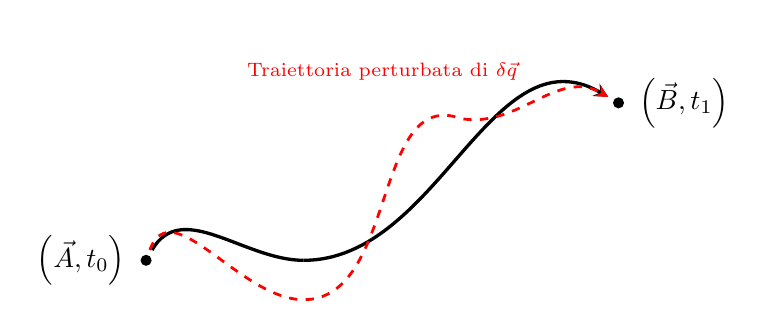
\begin{tikzpicture}[>=stealth, thick]

% Punti A e B
\node[label=left:{$\left(\vec{A}, t_0\right)$}] (A) at (0,0) {};
\node[label=right:{$\left(\vec{B}, t_1\right)$}] (B) at (6,2) {};

% Traiettoria principale (nera)
\draw[line width=1.2pt] (A) to[out=60, in=180] (2,0);
\draw[->, line width=1.2pt] (2,0) to[out=0, in=150] (B);

% Curva perturbata (rossa, composta da 3 tratti curvi)
\draw[->, red, dashed, line width=1pt]
  (A)
    to[out=70, in=180] (2,-0.5)
    to[out=0, in=160] (4,1.8)
    to[out=-10, in=150] (B);

% Punti visibili
\fill (A) circle (2pt);
\fill (B) circle (2pt);

% Etichetta facoltativa
\node[red] at (3,2.4) {\scriptsize Traiettoria perturbata di $\delta\vec{q}$ };

\end{tikzpicture}

    \caption{Perturbazione della traiettoria}
    \label{fig:1_TraiettoriaPertu}
\end{figure}

    }
    \caption{Perturbazione della traiettoria}
    \label{fig:1_TraiettoriaPertu}
\end{figure}


Siccome le variazioni di spostamento e velocità sono molto minori delle rispettive quantità (ovvero $\delta\mathbf{q}$ è una piccola variazione della traiettoria fisica):

\[
\delta q_{i} \ll q_{i} \quad \text{e} \quad \delta \dot{q}_{i} \ll \dot{q}_{i}
\]

è possibile sviluppare la lagrangiana $L$ in serie di Taylor, arrestando lo sviluppo al primo ordine, nell'intorno del punto \(\left( \mathbf{q},\mathbf{\dot{q}} \right)\). La variazione della Lagrangiana $\delta L$ è:

\[
L\left( \mathbf{q} + \delta\mathbf{q},\mathbf{\dot{q}} + \delta\mathbf{\dot{q}}, t \right) \simeq L\left( \mathbf{q},\mathbf{\dot{q}}, t \right) + \sum_{i=1}^s \left( \dfrac{\partial L}{\partial q_i}\delta q_i + \dfrac{\partial L}{\partial\dot{q}_i}\delta \dot{q}_i \right)
\]

Per comodità, si può esprimere la variazione $\delta L$ usando la notazione vettoriale (prodotto scalare generalizzato):

\[
L\left( \mathbf{q} + \delta\mathbf{q},\mathbf{\dot{q}} + \delta\mathbf{\dot{q}}, t \right) \simeq L\left( \mathbf{q},\mathbf{\dot{q}}, t \right) + \dfrac{\partial L}{\partial\mathbf{q}} \cdot \delta\mathbf{q} + \dfrac{\partial L}{\partial\mathbf{\dot{q}}}\cdot \delta\mathbf{\dot{q}}
\]

Sostituendo nell'espressione della variazione dell'azione, si ottiene:

\[
S + \delta S = \int_{t_{0}}^{t_{1}}{\left\lbrack L\left( \mathbf{q},\mathbf{\dot{q}}, t \right) + \dfrac{\partial L}{\partial\mathbf{q}}\delta\mathbf{q} + \dfrac{\partial L}{\partial\mathbf{\dot{q}}}\ \delta\mathbf{\dot{q}} \right\rbrack dt}
\]

Per la linearità dell'integrale si scrive:

\[
S + \delta S = \int_{t_{0}}^{t_{1}}{L\left( \mathbf{q},\mathbf{\dot{q}}, t \right)dt} + \int_{t_{0}}^{t_{1}}{\left( \dfrac{\partial L}{\partial\mathbf{q}}\delta\mathbf{q} + \dfrac{\partial L}{\partial\mathbf{\dot{q}}}\ \delta\mathbf{\dot{q}} \right)dt}
\]

Poiché:

\[
S = \int_{t_{0}}^{t_{1}}{L\left( \mathbf{q},\mathbf{\dot{q}}, t \right)dt}
\]

semplificando \(S\), si ottiene l'espressione per la variazione dell'azione \(\delta S\):

\[
\delta S = \int_{t_{0}}^{t_{1}}{\left( \dfrac{\partial L}{\partial\mathbf{q}}\delta\mathbf{q} + \dfrac{\partial L}{\partial\mathbf{\dot{q}}}\ \delta\mathbf{\dot{q}} \right)dt}
\]

La traiettoria perturbata $\mathbf{q} + \delta\mathbf{q}$ ha in comune con la traiettoria fisica $\mathbf{q}$ i punti iniziali e finali:

\[
\begin{cases}
\mathbf{q}\left( t_{0} \right) + \delta\mathbf{q}\left( t_{0} \right) = \mathbf{q}\left( t_{0} \right) \\
\mathbf{q}\left( t_{1} \right) + \delta\mathbf{q}\left( t_{1} \right) = \mathbf{q}\left( t_{1} \right)
\end{cases}
\]

Ne discende che la variazione deve essere nulla agli estremi temporali:

\[
\delta\mathbf{q}\left( t_{0} \right) = \mathbf{0},\quad\delta\mathbf{q}\left( t_{1} \right) = \mathbf{0}
\]

Poiché la variazione e la derivata temporale sono operazioni interscambiabili, risulta che:

\[
\delta\mathbf{\dot{q}} = \dfrac{d}{dt}\left( \delta\mathbf{q} \right)
\]

Dunque, la variazione di azione può essere espressa come:

\[
\delta S = \int_{t_{0}}^{t_{1}}{\dfrac{\partial L}{\partial\mathbf{q}}\delta\mathbf{q}dt} + \int_{t_{0}}^{t_{1}}{\dfrac{\partial L}{\partial\mathbf{\dot{q}}}\ \dfrac{d}{dt}\left( \delta\mathbf{q} \right)dt}
\]

Si integra per parti il secondo termine, del tipo:

\[
\int \mathbf{u} d\mathbf{v} = [\mathbf{uv}] - \int \mathbf{v} d\mathbf{u}
\]

Posto:

\[
\begin{cases}
\mathbf{u} = \dfrac{\partial L}{\partial\mathbf{\dot{q}}} \\
d\mathbf{v} = \dfrac{d}{dt}(\delta\mathbf{q}) dt
\end{cases}
\]

si ottiene:

\[
\int_{t_{0}}^{t_{1}}{\dfrac{\partial L}{\partial\mathbf{\dot{q}}}\ \dfrac{d}{dt}\left( \delta\mathbf{q} \right)dt} = \left\lbrack \dfrac{\partial L}{\partial\mathbf{\dot{q}}}\delta\mathbf{q} \right\rbrack_{t_{0}}^{t_{1}} - \int_{t_{0}}^{t_{1}}{\left( \dfrac{d}{dt}\dfrac{\partial L}{\partial\mathbf{\dot{q}}} \right)\delta\mathbf{q}dt}
\]


Grazie alle condizioni al contorno nulle ($\delta\mathbf{q}\left( t_{0} \right) = \delta\mathbf{q}\left( t_{1} \right) = \mathbf{0}$), il termine integrato è nullo:

\[
\left[\dfrac{\partial L}{\partial\mathbf{\dot{q}}}\delta\mathbf{q} \right]_{t_{0}}^{t_{1}} = 0
\]

Sostituendo nel $\delta S$ si ottiene:

\[
\delta S = \int_{t_{0}}^{t_{1}}{\dfrac{\partial L}{\partial\mathbf{q}}\delta\mathbf{q}dt} - \int_{t_{0}}^{t_{1}}{\left( \dfrac{d}{dt}\dfrac{\partial L}{\partial\mathbf{\dot{q}}} \right)\delta\mathbf{q}dt}
\]

Raccogliendo $\delta\mathbf{q}$ (che è una moltiplicazione scalare dei due vettori):

\[
\delta S = \int_{t_{0}}^{t_{1}}{\left( \dfrac{\partial L}{\partial\mathbf{q}} - \dfrac{d}{dt}\dfrac{\partial L}{\partial\mathbf{\dot{q}}} \right)\delta\mathbf{q}dt}
\]

Dato che l'azione deve essere stazionaria, la sua variazione deve essere nulla \(\delta S = 0\). Per cui si ha:

\[
\int_{t_{0}}^{t_{1}}{\left( \dfrac{\partial L}{\partial\mathbf{q}} - \dfrac{d}{dt}\dfrac{\partial L}{\partial\mathbf{\dot{q}}} \right)\delta\mathbf{q}dt} = 0
\]

Poiché $\delta\mathbf{q}$ è una variazione arbitraria e non nulla all'interno dell'intervallo ($\left[t_0; \ t_1\right]$), il Lemma Fondamentale del Calcolo delle Variazioni stabilisce che il coefficiente di $\delta\mathbf{q}$ deve essere il vettore nullo:

\[
\dfrac{d}{dt}\dfrac{\partial L}{\partial\mathbf{\dot{q}}} - \dfrac{\partial L}{\partial\mathbf{q}} = \mathbf{0}
\]

Questa è l'Equazione di \textbf{Eulero-Lagrange in forma vettoriale}, che equivale a $s$ equazioni scalari differenziali del secondo ordine.

\subsubsection{Particella in coordinate cartesiane}\label{particella-in-coordinate-cartesiane}

Per una \textbf{particella libera} (cioè in assenza di forze  e non conservative, dove l'energia potenziale è nulla) in moto in uno spazio cartesiano, la lagrangiana \(L\) è data da:

\[
L = \dfrac{1}{2}mv^{2}
\]

Dove

\[
v^{2} = {\dot{x}}^{2} + {\dot{y}}^{2} + {\dot{z}}^{2}
\]

In altre parole, in questo caso la lagrangiana coincide con l'energia cinetica della particella. Inoltre, la descrizione lagrangiana si riduce alla modellazione newtoniana, dato che il sistema di riferimento corrisponde con quello cartesiano. Tuttavia, nella pratica non è sempre conveniente descrivere il moto in coordinate cartesiane. In presenza di vincoli o geometrie particolari, infatti, è utile ricorrere alle coordinate generalizzate \(\mathbf{q}\) e \(\mathbf{\dot{q}}\). È quindi necessario esprimere l'energia del sistema in funzione di queste coordinate.

\subsection{Energia cinetica in coordinate generalizzate}\label{energia-cinetica-in-generalizzate}

Per un sistema di \(N\) particelle nelle coordinate generalizzate \(\mathbf{q}\) e \(\mathbf{\dot{q}}\), l'energia cinetica $T$ è data da:

\[
T = T\left( \mathbf{q},{\dot{\mathbf{q}}}, t \right)
\]

In un sistema scleronomo (vincoli indipendenti dal tempo), l'energia cinetica è una forma quadratica omogenea nelle velocità generalizzate, e dunque è una funzione di \( \mathbf{q} \) e \( \mathbf{\dot{q}} \).

Si considerano le funzioni vettoriali $\mathbf{r}_{i}$ che legano le coordinate cartesiane di ciascuna particella $\mathbf{r}_{i} = (x_{i},y_{i},z_{i})$ con le coordinate generalizzate $ \mathbf{q} = (q_{1},q_{2},\ldots,q_{s}) $.

\[
\mathbf{r}_{i} = \mathbf{r}_{i}\left( q_{1},\ q_{2},\ \ldots,\ q_{s}, t \right),\quad i = 1,2,\ldots,N
\]

Si deriva $\mathbf{r}_{i}$ rispetto al tempo per ottenere la velocità $\mathbf{\dot{r}}_{i}$:

\[
\mathbf{\dot{r}}_{i} = \dfrac{d\mathbf{r}_{i}}{dt} = \sum_{k = 1}^{s}{\dfrac{\partial \mathbf{r}_{i}}{\partial q_{k}}\dfrac{dq_{k}}{dt}} + \dfrac{\partial \mathbf{r}_{i}}{\partial t} = \sum_{k = 1}^{s}{\dfrac{\partial \mathbf{r}_{i}}{\partial q_{k}}{\dot{q}}_{k}} + \dfrac{\partial \mathbf{r}_{i}}{\partial t}
\]

Per semplicità, consideriamo il caso scleronomo, dove le variazioni temporali dei vincoli sono nulle:

\[
{\mathbf{\dot{r}}}_{i} = \sum_{k = 1}^{s}{\dfrac{\partial \mathbf{r}_{i}}{\partial q_{k}}{\dot{q}}_{k}}
\]

Si eleva al quadrato ${\mathbf{\dot{r}}}_{i}$, mediante prodotto scalare, ottenendo:

\[
\dot{r}_{i}^{2} = {\mathbf{\dot{r}}}_{i} \cdot {\mathbf{\dot{r}}}_{i} = \left( \sum_{k = 1}^{s}{\dfrac{\partial \mathbf{r}_{i}}{\partial q_{k}}{\dot{q}}_{k}} \right) \cdot \left( \sum_{j = 1}^{s}{\dfrac{\partial \mathbf{r}_{i}}{\partial q_{j}}{\dot{q}}_{j}} \right)
\]
È possibile esprimere il secondo membro come doppia sommatoria sugli indici \(k\) e \(j\):

\[
\dot{r}_{i}^{2} = \sum_{k = 1}^{s}{\sum_{j = 1}^{s}{\left(\dfrac{\partial \mathbf{r}_{i}}{\partial q_{j}}\cdot \dfrac{\partial \mathbf{r}_{i}}{\partial q_{k}}\right){\dot{q}}_{j}}{\dot{q}}_{k}}
\]

L'energia cinetica totale del sistema è:

\[
T = \dfrac{1}{2}\sum_{i = 1}^{N}{m_{i}{\dot{r}}}_{i}^{2}
\]

Sostituendo in quest'ultima espressione ${\dot{r}}_{i}^{2}$:

\[
T = \dfrac{1}{2}\sum_{k = 1}^{s}{\sum_{j = 1}^{s}\left(\sum_{i = 1}^{N}{m_{i}\dfrac{\partial \mathbf{r}_{i}}{\partial q_{j}}\cdot \dfrac{\partial \mathbf{r}_{i}}{\partial q_{k}}}\right){\dot{q}}_{k}{\dot{q}}_{j}}
\]

Si definiscono i coefficienti metrici della massa generalizzata:

\[
a_{kj}(\mathbf{q}) = \sum_{i = 1}^{N}{m_{i}\dfrac{\partial \mathbf{r}_{i}}{\partial q_{j}}\cdot \dfrac{\partial \mathbf{r}_{i}}{\partial q_{k}}}
\]

Allora l'energia cinetica può essere scritta come forma quadratica nelle velocità generalizzate:

\[T = \dfrac{1}{2}\sum_{k = 1}^{s}{\sum_{j = 1}^{s}a_{kj}(\mathbf{q}){\dot{q}}_{k}{\dot{q}}_{j}}\]

Dato che \(a_{kj}\) è un parametro dipendente dalla posizione generalizzata $\mathbf{q}$, l'energia cinetica totale dipende dalla velocità e dalla posizione generalizzate.

\subsection{Energia potenziale in coordinate generalizzate}\label{energia-potenziale-in-coordinate-generalizzate}
È conveniente esprimere anche l'energia potenziale in funzione delle coordinate generalizzate. Si considera un sistema di \(N\) particelle. L'energia di interazione tra le particelle è indicata con \(U(\mathbf{q})\) e viene denotata come energia potenziale. In meccanica classica, per forze conservative, questa quantità dipende solamente dalla posizione generalizzata. In particolare, se le coordinate generalizzate $\mathbf{q}$ descrivono completamente la configurazione del sistema, allora l'energia potenziale può essere scritta come:

\[
U = U(q_{1},q_{2},\ldots,q_{s})
\]

dove \(s\) è il numero di coordinate generalizzate.

La meccanica classica assume che le interazioni tra le particelle avvengano istantaneamente (ovvero che il potenziale sia indipendente dalla velocità), non considerando gli effetti di propagazione dei cambiamenti nei campi di forza. Tuttavia, secondo la teoria della relatività di Einstein, le interazioni si propagano attraverso campi con velocità finita, non superiore alla velocità della luce \(c\). Questo implica che la descrizione classica è un'approssimazione valida solo quando le velocità coinvolte sono molto inferiori a \(c\) e gli effetti di ritardo possono essere trascurati.

\subsection{Espressione della lagrangiana}\label{espressione-della-lagrangiana}
La lagrangiana è la funzione scalare definita come la differenza tra l'energia cinetica \(T\) e l'energia potenziale \(U\), secondo la relazione \cite{arnold1992matematici, landau1994meccanica}:

\[
L\left( \mathbf{q},\mathbf{\dot{q}}, t \right) = T\left( \mathbf{q},\mathbf{\dot{q}}, t \right) - U\left( \mathbf{q}, t \right)
\]

dove \(s\) è il numero di gradi di libertà del sistema.

In un sistema scleronomo (vincoli indipendenti dal tempo) e con potenziale indipendente dal tempo ($U=U(\mathbf{q})$), la Lagrangiana non dipende esplicitamente dal tempo $t$:

\[
L\left( \mathbf{q},\mathbf{\dot{q}} \right) = T\left( \mathbf{q},\mathbf{\dot{q}} \right) - U\left( \mathbf{q} \right)
\]

La lagrangiana \(L\) è, dunque, una funzione delle coordinate generalizzate di posizione e velocità, che a loro volta dipendono dal tempo:

\[
L : TQ \times \mathbb{R} \rightarrow \mathbb{R}
\]

dove \(Q\) è lo \textbf{spazio delle configurazioni} e \(TQ\) indica il \textbf{fibrato tangente} dello spazio delle configurazioni, dove:

\begin{itemize}
\item Un elemento di \(Q\) è semplicemente una configurazione $\mathbf{q}$;
\item Un elemento di \(TQ\) è una coppia \(\left( \mathbf{q},\mathbf{\dot{q}} \right)\), che rappresenta la posizione (o configurazione) e la velocità generalizzata del sistema.
\end{itemize}

Se la lagrangiana non dipende esplicitamente dal tempo (sistema olonomo e scleronomo con potenziale statico) essa agisce sul fibrato tangente a valori in \(\mathbb{R}\):

\[
L : TQ \rightarrow \mathbb{R}
\]

Si considera l'azione \(S\), data per definizione da:

\[
S = \int_{t_{1}}^{t_{2}}{L\left( \mathbf{q},\mathbf{\dot{q}}, t \right)dt}
\]

L'azione dipende dalle coordinate generalizzate, funzioni del tempo, dunque, è un funzionale poiché associa a ogni funzione $\mathbf{q}(t)$ un valore numerico. Dunque, l'azione è definita nello spazio vettoriale delle traiettorie generalizzate $\mathbb{V =}\left\{ \mathbf{q}(t) \right\}$ a valori in \(\mathbb{R}\):

\[
S:\mathbb{V} \rightarrow \mathbb{R}
\]

\subsection{Legame tra lagrangiana ed equazioni di Newton}\label{legame-tra-lagrangiana-ed-equazioni-di-newton}

Per individuare una correlazione tra la meccanica newtoniana e quella lagrangiana si scrive l'equazione di Eulero-Lagrange in coordinate cartesiane. In generale, l'equazione di Eulero-Lagrange per la $i$-esima coordinata generalizzata è:

\[
\dfrac{d}{dt}\dfrac{\partial L}{\partial{\dot{q}}_{i}} - \dfrac{\partial L}{\partial q_{i}} = 0
\]

È noto che la lagrangiana è data da:

\[
L\left( \mathbf{q},\mathbf{\dot{q}}, t \right) = T\left( \mathbf{q},\mathbf{\dot{q}}, t \right) - U\left( \mathbf{q}, t \right)
\]

Per cui, è possibile scrivere l'equazione in termini di energie:

\[
\dfrac{d}{dt}\dfrac{\partial}{\partial{\dot{q}}_{i}}\left[ T\left( \mathbf{q},\mathbf{\dot{q}} \right) - U\left( \mathbf{q} \right) \right] - \dfrac{\partial}{\partial q_{i}}\left[ T\left( \mathbf{q},\mathbf{\dot{q}} \right) - U\left( \mathbf{q} \right) \right] = 0
\]

Si considera il caso in cui le coordinate generalizzate coincidano con le coordinate cartesiane di tutte le particelle, ovvero $q_i = x_i$. In questo caso, le coordinate sono indipendenti ($s=3N$). La Lagrangiana in coordinate cartesiane $\mathbf{x} = (x_1, \ldots, x_{3N})$ è:

\[
L\left( \mathbf{x},\mathbf{\dot{x}} \right) = T\left( \mathbf{\dot{x}} \right) - U\left( \mathbf{x} \right)
\]

dove l'energia cinetica $T$ dipende solo dalle velocità e l'energia potenziale $U$ dipende solo dalle posizioni.

L'equazione di Eulero-Lagrange in coordinate cartesiane $x_i$ diventa:

\[
\dfrac{d}{dt}\dfrac{\partial}{\partial{\dot{x}}_{i}}\left[ T\left( \mathbf{\dot{x}} \right) - U\left( \mathbf{x} \right) \right] - \dfrac{\partial}{\partial x_{i}}\left[ T\left( \mathbf{\dot{x}} \right) - U\left( \mathbf{x} \right) \right] = 0
\]

Sfruttando le dipendenze dei termini energetici in coordinate cartesiane:

\[
\dfrac{\partial U}{\partial \dot{x}_i} = 0 \quad \text{e} \quad \dfrac{\partial T}{\partial x_i} = 0
\]

Si ottiene:

\[
\dfrac{d}{dt}\dfrac{\partial T}{\partial{\dot{x}}_{i}} - \left( - \dfrac{\partial U}{\partial x_{i}} \right) = 0 \Leftrightarrow \dfrac{d}{dt}\dfrac{\partial T}{\partial{\dot{x}}_{i}} = - \dfrac{\partial U}{\partial x_{i}}
\]

L'energia cinetica per un sistema di \(N\) particelle, in coordinate cartesiane, è:

\[
T = \dfrac{1}{2}\sum_{j = 1}^{3N}{m_{j}{\dot{x}}_{j}^{2}}
\]

Applicando la derivata parziale rispetto a \({\dot{x}}_{i}\) si ottiene il momento coniugato cartesiano $p_i$:

\[
\dfrac{\partial T}{\partial{\dot{x}}_{i}} = \dfrac{\partial}{\partial{\dot{x}}_{i}}\left( \dfrac{1}{2}\sum_{j = 1}^{3N}{m_{j}{\dot{x}}_{j}^{2}} \right) = m_{i}{\dot{x}}_{i} = p_i
\]

Derivando quantità rispetto al tempo si ottiene il primo membro dell'equazione di Eulero-Lagrange in coordinate cartesiane:

\[
\dfrac{d}{dt}\dfrac{\partial T}{\partial{\dot{x}}_{i}} = \dfrac{d}{dt}\left( m_{i}{\dot{x}}_{i} \right) = m_{i}{\ddot{x}}_{i}
\]

Sostituendo nell'equazione di Eulero-Lagrange si ottiene l'Equazione di Newton per la coordinata $x_i$:

\[
\dfrac{d}{dt}\dfrac{\partial T}{\partial{\dot{x}}_{i}} = - \dfrac{\partial U}{\partial x_{i}} \Leftrightarrow m_{i}{\ddot{x}}_{i} = - \dfrac{\partial U}{\partial x_{i}}
\]

Dal secondo principio della dinamica è noto che:

\[
m_{i}{\ddot{x}}_{i} = F_{i}
\]

dove $F_{i}$ è la $i$-esima componente della forza conservativa agente sulla particella. Poiché la forza conservativa è data dal gradiente negativo dell'energia potenziale ($\mathbf{F} = -\mathbf{\nabla}U$):

\[
F_{i} = - \dfrac{\partial U}{\partial x_{i}}
\]

La Lagrangiana è quindi equivalente alle leggi di Newton (per sistemi conservativi). 

Va notato che in coordinate cartesiane, l'energia potenziale non dipende dalla velocità, dunque:

\[
\dfrac{\partial T}{\partial{\dot{x}}_{i}} = \dfrac{\partial}{\partial{\dot{x}}_{i}}\left(L + U\right) = \dfrac{\partial L}{\partial{\dot{x}}_{i}}
\]

Si ottiene:

\[
\dfrac{\partial L}{\partial{\dot{x}}_{i}} = {p}_i
\]

Ne discende che la quantità di moto $p_{i}$ e la forza $F_{i}$ sono legate alla Lagrangiana $L$ e all'energia potenziale $U$ dalle relazioni generali \cite{arnold1992matematici, landau1994meccanica}:

\[
\begin{cases}
p_{i} = \dfrac{\partial L}{\partial{\dot{q}}_{i}} & \quad (\text{Momento generalizzato coniugato}) \\
Q_{i} = - \dfrac{\partial U}{\partial q_{i}} & \quad (\text{Forza generalizzata conservativa})
\end{cases}
\]

Le due relazioni sono note come definizioni fondamentali della meccanica lagrangiana. La prima (\(p_{i}\)) è detta \textbf{momento generalizzato coniugato}, mentre la seconda forza generalizzata. 

Più in generale, la \textbf{forza generalizzata} $Q_i$ è definita come il coefficiente del lavoro virtuale $\delta W = \sum_i Q_i \delta q_i$:

\[
Q_i = \sum_j \mathbf{F}_j \cdot \frac{\partial \mathbf{r}_j}{\partial q_i}
\]

Considerando l'equazione di Eulero-Lagrange e sostituendo la relazione per il momento coniugato generalizzato:

\[\dfrac{d}{dt}\dfrac{\partial L}{\partial{\dot{q}}_{i}} - \dfrac{\partial L}{\partial q_{i}} = 0 \quad \Leftrightarrow \quad \dfrac{d}{dt}p_{i} = \dfrac{\partial L}{\partial q_{i}}\]

Da cui risulta:

\[
\dot{p}_{i} = \dfrac{\partial L}{\partial q_{i}}
\]

Questa relazione lega la derivata del momento generalizzato coniugato alla Lagrangiana ed è centrale in Meccanica Hamiltoniana.

\subsection{Principio di conservazione}\label{principio-di-conservazione}

Le leggi di conservazione dell'energia, del momento lineare e del momento angolare sono una conseguenza delle simmetrie fondamentali dello spazio e del tempo. In particolare, queste leggi di conservazione sono connesse all'invarianza delle leggi fisiche del sistema rispetto a determinate trasformazioni. Questo legame profondo fu dimostrato da Emmy Noether nel 1915 \cite{arnold1992matematici}. Secondo il suo teorema, a ogni simmetria continua e differenziabile delle leggi fisiche corrisponde una quantità conservata:

\begin{itemize}
\item
 Dall'omogeneità temporale discende la conservazione dell'energia. L'omogeneità temporale implica che le leggi fisiche non cambiano se un fenomeno viene traslato nel tempo;
\item
 Dall'omogeneità spaziale deriva la conservazione del momento lineare (o quantità di moto). L'omogeneità spaziale implica che le leggi fisiche non variano se il sistema viene traslato nello spazio;
\item
 Dall'isotropia dello spazio discende la conservazione del momento angolare. L'isotropia spaziale implica che le leggi fisiche non cambiano se il sistema viene ruotato nello spazio.
\end{itemize}

\subsection{Conservazione dell'energia}\label{conservazione-dellenergia}

L'energia totale $E=T+U$ si conserva grazie alla proprietà di omogeneità temporale. La conservazione dell'energia si verifica se la Lagrangiana non dipende esplicitamente dal tempo:

\[
\dfrac{\partial L}{\partial t} = 0
\]

In questo caso, il sistema è isolato e scleronomo. La Lagrangiana dipende dal tempo solo attraverso le coordinate generalizzate \cite{landau1994meccanica}: 

\[
L = L\left( \mathbf{q},\mathbf{\dot{q}} \right),\quad \mathbf{q} = \mathbf{q}\left(t\right),\mathbf{\dot{q}} = \mathbf{\dot{q}}\left(t\right)
\] 

La derivata totale rispetto al tempo della lagrangiana, per la derivata delle funzioni composte, è: 

\[ 
\dfrac{d L}{d t} = \sum_{i=1}^s \left( \dfrac{\partial L}{\partial q_i}\dfrac{d q_i}{d t} + \dfrac{\partial L}{\partial \dot{q}_i}\dfrac{d \dot{q}_i}{d t} \right) + \dfrac{\partial L}{\partial t} 
\] 

Poiché si assume che la lagrangiana non dipendente esplicitamente dal tempo la sua derivata rispetto a tale variabile è nulla. Utilizzando la notazione vettoriale, mediante il prodotto scalare generalizzato, è possibile scrivere: 

\[ 
\dfrac{d L}{d t} = \dfrac{\partial L}{\partial\mathbf{q}}\cdot\mathbf{\dot{q}} + \dfrac{\partial L}{\partial\mathbf{\dot{q}}}\cdot\mathbf{\ddot{q}} 
\] 

Dalle equazioni di Eulero-Lagrange, si ha che:

\[
\dfrac{d}{dt}\left( \dfrac{\partial L}{\partial\mathbf{\dot{q}}} \right) - \dfrac{\partial L}{\partial\mathbf{q}} = 0 \Leftrightarrow \dfrac{\partial L}{\partial\mathbf{q}} = \dfrac{d}{dt}\left( \dfrac{\partial L}{\partial\mathbf{\dot{q}}} \right)
\]

Sostituendo nella derivata totale della Lagrangiana: 

\[ 
\dfrac{d L}{d t} = \dfrac{d}{dt}\left( \dfrac{\partial L}{\partial\mathbf{\dot{q}}} \right)\cdot\mathbf{\dot{q}} + \dfrac{\partial L}{\partial\mathbf{\dot{q}}}\cdot\mathbf{\ddot{q}} 
\] 

Si osserva che il secondo membro è esattamente la derivata totale rispetto al tempo del prodotto scalare (Regola di Leibniz per il prodotto scalare): 

\[ 
\dfrac{d}{dt}\left( \dfrac{\partial L}{\partial\mathbf{\dot{q}}}\cdot\mathbf{\dot{q}} \right) = \dfrac{d}{dt}\left( \dfrac{\partial L}{\partial\mathbf{\dot{q}}} \right)\cdot\mathbf{\dot{q}} + \dfrac{\partial L}{\partial\mathbf{\dot{q}}}\cdot\dfrac{d\mathbf{\dot{q}}}{dt} 
\] 

Dunque, si ottiene: 
\[ 
\dfrac{d L}{d t} = \dfrac{d}{dt}\left( \dfrac{\partial L}{\partial\mathbf{\dot{q}}}\cdot\mathbf{\dot{q}} \right) 
\] 

Portando tutto a sinistra, si ha: 
\[ 
\dfrac{d}{dt}\left( L - \dfrac{\partial L}{\partial\mathbf{\dot{q}}}\cdot\mathbf{\dot{q}} \right) = 0 
\] 

Si definisce l'Hamiltoniana o Energia del sistema $H$ come la quantità: 

\[ 
H = \dfrac{\partial L}{\partial\mathbf{\dot{q}}}\cdot\mathbf{\dot{q}} - L 
\]

Poiché la derivata temporale dell'Hamiltoniana è nulla, si conclude che $H$ è una costante del moto (conservata): 

\[
\dfrac{d H}{d t} = 0 \Leftrightarrow H = \text{cost} 
\]

Per definizione di lagrangiana, risulta che:

\[
L = T - U
\]

L'energia potenziale $U$ non dipende dalle velocità generalizzate $\mathbf{\dot{q}}$. Dunque,  risulta:

\[
\dfrac{\partial L}{\partial \dot{q}_i} = \dfrac{\partial}{\partial \dot{q}_i}(T - U) = \dfrac{\partial T}{\partial \dot{q}_i}
\]

Per i sistemi scleronomi (dove i vincoli non dipendono esplicitamente dal tempo), l'energia cinetica $T$ è una forma quadratica omogenea nelle velocità generalizzate $\mathbf{\dot{q}}$. Sfruttando la struttura di $T$:

\[ 
T = \dfrac{1}{2}\sum_{k, j} a_{kj}(\mathbf{q}){\dot{q}}_{k}{\dot{q}}_{j} 
\]

dove i coefficienti $a_{kj}(\mathbf{q})$ sono simmetrici, ovvero $a_{kj} = a_{jk}$. 

Si deriva $T$ rispetto a una specifica velocità generalizzata $\dot{q}_i$. Nella doppia sommatoria, la derivata parziale è non nulla solo quando $i$ compare come indice $k$ o come indice $j$. 
 
\[ 
\dfrac{\partial T}{\partial \dot{q}_i} = \dfrac{1}{2} \sum_{k, j} a_{kj} \dfrac{\partial}{\partial \dot{q}_i} (\dot{q}_k \dot{q}_j) 
\] 

Usando la regola di derivazione e ricordando che:

\[
\dfrac{\partial \dot{q}_k}{\partial \dot{q}_i} = \delta_{ik} \quad \text{e} \quad \dfrac{\partial \dot{q}_j}{\partial \dot{q}_i} = \delta_{ij}
\]

è possibile scrivere:

\[ 
\dfrac{\partial T}{\partial \dot{q}_i} = \dfrac{1}{2} \sum_{k, j} a_{kj} \left( \delta_{ik} \dot{q}_j + \dot{q}_k \delta_{ij} \right) 
\]

La presenza del $\delta_{ik}$ annulla la sommatoria su $k$ eccetto quando $k=i$; il $\delta_{ij}$ annulla la sommatoria su $j$ eccetto quando $j=i$:

\[ 
\dfrac{\partial T}{\partial \dot{q}_i} = \dfrac{1}{2} \left[ \sum_{j} a_{ij} \dot{q}_j + \sum_{k} a_{ki} \dot{q}_k \right] 
\]

Poiché i coefficienti sono simmetrici ($a_{ij} = a_{ji}$), le due sommatorie sono identiche. Dunque:

\[ 
\dfrac{\partial T}{\partial \dot{q}_i} = \dfrac{1}{2} \left[ 2 \sum_{j=1}^{s} a_{ij} \dot{q}_j \right] = \sum_{j=1}^{s} a_{ij} \dot{q}_j 
\] 

Moltiplichiamo il risultato della prima relazione per $\dot{q}_i$ e sommiamo su tutti gli indici $i$ (ottenendo il prodotto scalare $\dfrac{\partial T}{\partial\mathbf{\dot{q}}}\cdot\mathbf{\dot{q}}$): 
 
\[ 
\sum_{i=1}^{s} \dfrac{\partial T}{\partial \dot{q}_i} \dot{q}_i = \sum_{i=1}^{s} \dot{q}_i \left( \sum_{j=1}^{s} a_{ij} \dot{q}_j \right) 
\]

Riordinando la doppia sommatoria: 
 
\[ 
\sum_{i=1}^{s} \dfrac{\partial T}{\partial \dot{q}_i} \dot{q}_i = \sum_{i=1}^{s} \sum_{j=1}^{s} a_{ij} \dot{q}_i \dot{q}_j 
\]

Confrontando il risultato finale con la formula originale di $T$: 
 
\[ 
T = \dfrac{1}{2}\sum_{i=1}^{s}{\sum_{j = 1}^{s}a_{ij}{\dot{q}}_{i}{\dot{q}}_{j}} 
\] 
 
Si ottiene immediatamente la relazione cercata: 
 
\[ 
\dfrac{\partial T}{\partial\mathbf{\dot{q}}}\cdot\mathbf{\dot{q}} = \sum_{i=1}^{s} \dfrac{\partial T}{\partial \dot{q}_i} \dot{q}_i = 2 \left[ \dfrac{1}{2}\sum_{i=1}^{s} \sum_{j=1}^{s} a_{ij} \dot{q}_i \dot{q}_j \right] = 2T 
\] 

Tale risultato è noto come \textbf{Teorema di Eulero}. Sostituendo nell'espressione per $H$: 
 
\[ 
H = \left(\dfrac{\partial T}{\partial\mathbf{\dot{q}}}\cdot\mathbf{\dot{q}}\right) - L = 2T - (T - U) = T + U 
\] 

In definitiva, si è dimostrato che la conservazione dell'energia totale (\(E = T+U\)) è una diretta conseguenza della simmetria temporale (omogeneità temporale) delle leggi fisiche.

\subsection{Conservazione della quantità di moto}\label{conservazione-della-quantituxe0-di-moto}

Il momento lineare totale del sistema è: 
 
\[ 
\mathbf{P} = \sum_{i = 1}^{N}{\mathbf{p}}_{i} = \sum_{i = 1}^{N}{m_i \mathbf{v}}_{i} 
\]

Esso si conserva grazie alla proprietà di \textbf{omogeneità spaziale}. L'omogeneità spaziale implica che le leggi fisiche del sistema non devono cambiare se il sistema viene traslato uniformemente nello spazio.

Si considera una traslazione infinitesima e uniforme $\delta \mathbf{r}$ che agisce su tutte le coordinate cartesiane $\mathbf{r}_i$ delle $N$ particelle: 

\[ 
\mathbf{r}_i \to \mathbf{r}_i + \delta \mathbf{r} \quad (\text{dove } \delta \mathbf{r} \text{ è lo stesso per tutti gli } i) 
\]

La Lagrangiana $L(\mathbf{r}_i, \mathbf{v}_i)$ non deve cambiare per questa traslazione, per l'ipotesi di omogeneità spaziale, quindi $\delta L = 0$ \cite{landau1994meccanica}.

\[ 
\delta L = \sum_{i=1}^N \dfrac{\partial L}{\partial \mathbf{r}_i} \cdot \delta \mathbf{r}_i + \sum_{i=1}^N \dfrac{\partial L}{\partial \mathbf{v}_i} \cdot \delta \mathbf{v}_i 
\]

Poiché la traslazione è uniforme:
\[
\delta \mathbf{v}_i = \dfrac{d}{dt}(\delta \mathbf{r}) = \mathbf{0}
\]

Sostituendo $\delta \mathbf{r}_i = \delta \mathbf{r}$:

\[ 
\delta L = \left( \sum_{i=1}^N \dfrac{\partial L}{\partial \mathbf{r}_i} \right) \cdot \delta \mathbf{r} 
\]

L'omogeneità spaziale impone $\delta L = 0$ per una traslazione arbitraria $\delta \mathbf{r}$, il che implica che la somma delle derivate sia nulla: 

\[ 
\sum_{i=1}^N \dfrac{\partial L}{\partial \mathbf{r}_i} = \mathbf{0} 
\]

Applichiamo l'equazione di Eulero-Lagrange in coordinate cartesiane $\mathbf{r}_i$:

\[ 
\dfrac{\partial L}{\partial \mathbf{r}_i} = \dfrac{d}{dt}\left( \dfrac{\partial L}{\partial \mathbf{v}_i} \right) 
\] 

Sommando su tutte le particelle $i=1, \ldots, N$:

\[ 
\sum_{i=1}^N \dfrac{\partial L}{\partial \mathbf{r}_i} = \sum_{i=1}^N \dfrac{d}{dt}\left( \dfrac{\partial L}{\partial \mathbf{v}_i} \right) 
\]

Sostituendo la condizione di omogeneità spaziale:
\[
\sum_{i=1}^N \dfrac{\partial L}{\partial \mathbf{r}_i} = \mathbf{0}
\]

si ottiene:

\[ 
\sum_{i=1}^N \dfrac{d}{dt}\left( \dfrac{\partial L}{\partial \mathbf{v}_i} \right) = \mathbf{0} 
\]

Per linearità è possibile commutare l'operatore di derivazione temporale con la sommatoria:

\[ 
\dfrac{d}{dt}\left( \sum_{i=1}^N \dfrac{\partial L}{\partial \mathbf{v}_i} \right) = \mathbf{0} 
\] 
 
Integrando rispetto al tempo si ottiene: 

\[ 
\sum_{i=1}^N \dfrac{\partial L}{\partial \mathbf{v}_i} = \mathbf{const} 
\] 

In altre parole, il gradiente della lagrangiana rispetto alla velocità è costante.

La Lagrangiana in coordinate cartesiane è: 

\[ 
L = \dfrac{1}{2}\sum_{i = 1}^{N}{m_{i} \mathbf{v}_{i} \cdot \mathbf{v}_{i}} - U\left( \mathbf{r}_{1}, \ldots, \mathbf{r}_{N} \right) 
\] 
 
Si calcola la derivata parziale rispetto alla velocità di una singola particella $\mathbf{v}_k$: 

\[ 
\dfrac{\partial L}{\partial \mathbf{v}_k} = \dfrac{\partial}{\partial \mathbf{v}_k} \left( \dfrac{1}{2}\sum_{i}{m_{i} \mathbf{v}_{i}^2} \right) - \dfrac{\partial U}{\partial \mathbf{v}_k} 
\] 

Poiché $U$ non dipende dalle velocità e la sommatoria è non nulla solo per $i=k$: 

\[ 
\dfrac{\partial L}{\partial \mathbf{v}_k} = m_k \mathbf{v}_k = \mathbf{p}_k 
\]

Sostituendo questo risultato nell'equazione di conservazione: 

\[ 
\sum_{i=1}^N \dfrac{\partial L}{\partial \mathbf{v}_i} = \sum_{i=1}^N \mathbf{p}_i = \mathbf{P} = \mathbf{const} 
\] 
 
La \textbf{quantità di moto totale} $\mathbf{P}$ si conserva in ipotesi di omogeneità spaziale. 

\subsection{Conservazione del momento angolare}\label{conservazione-del-momento-angolare}

Il momento angolare totale del sistema è definito come \cite{landau1994meccanica}:

\[ 
\mathbf{L} = \sum_{i = 1}^{N}{\mathbf{r}}_{i} \times {\mathbf{p}}_{i} 
\]

esso si conserva lungo le direzioni corrispondenti all'isotropia spaziale o a simmetrie parziali del potenziale $U$. Ad esempio, se il potenziale ha simmetria cilindrica, la proiezione del momento angolare lungo quest'asse si conserva.

Si suppone che lo spazio sia \textbf{isotropo} (o che il potenziale abbia simmetria rotazionale lungo un asse). Questo implica che una rotazione infinitesima $d\boldsymbol{\varphi}$ non deve modificare la Lagrangiana. La rotazione infinitesima induce variazioni sia nella posizione $\mathbf{r}_i$ sia nella velocità $\mathbf{v}_i$ di ciascuna particella $i$:

\[ 
\delta\mathbf{r}_{i} = d\boldsymbol{\varphi} \times \mathbf{r}_{i},\quad \delta\mathbf{v}_{i} = d\boldsymbol{\varphi} \times \mathbf{v}_{i} 
\]

La variazione totale $\delta L$ della Lagrangiana, per il caso di $N$ particelle, è data dal differenziale:

\[ 
\delta L = \sum_{i = 1}^{N}\left( \dfrac{\partial L}{\partial\mathbf{v}_{i}} \cdot \delta\mathbf{v}_{i} + \dfrac{\partial L}{\partial\mathbf{r}_{i}} \cdot \delta\mathbf{r}_{i} \right) 
\]

Per l'ipotesi di isotropia, la variazione deve essere nulla ($\delta L = 0$): 
 
\[ 
\sum_{i = 1}^{N}\left( \dfrac{\partial L}{\partial\mathbf{v}_{i}} \cdot \delta\mathbf{v}_{i} + \dfrac{\partial L}{\partial\mathbf{r}_{i}} \cdot \delta\mathbf{r}_{i} \right) = 0 
\] 

Sostituendo le espressioni per $\delta\mathbf{r}_{i}$ e $\delta\mathbf{v}_{i}$, si ottiene: 
 
\[ 
\sum_{i = 1}^{N}\left\lbrack \dfrac{\partial L}{\partial\mathbf{v}_{i}} \cdot \left( d\boldsymbol{\varphi} \times \mathbf{v}_{i} \right) + \dfrac{\partial L}{\partial\mathbf{r}_{i}} \cdot \left( d\boldsymbol{\varphi} \times \mathbf{r}_{i} \right) \right\rbrack = 0 
\]

Dati tre vettori generici \(\mathbf{a}\), \(\mathbf{b}\) e \(\mathbf{c}\), è valida la proprietà del triplo prodotto scalare ciclico (o prodotto misto): 

\[ 
\left( \mathbf{a} \times \mathbf{b} \right) \cdot \mathbf{c} = \left( \mathbf{b} \times \mathbf{c} \right) \cdot \mathbf{a} 
\]

si può isolare l'elemento infinitesimo di rotazione $d\boldsymbol{\varphi}$:
 
\[ 
\sum_{i = 1}^{N}\left[ d\boldsymbol{\varphi} \cdot \left( \mathbf{v}_{i} \times \dfrac{\partial L}{\partial\mathbf{v}_{i}} \right) + d\boldsymbol{\varphi} \cdot \left( \mathbf{r}_{i} \times \dfrac{\partial L}{\partial\mathbf{r}_{i}} \right) \right] = d\boldsymbol{\varphi} \cdot \sum_{i = 1}^{N}\left( \mathbf{v}_{i} \times \dfrac{\partial L}{\partial\mathbf{v}_{i}} + \mathbf{r}_{i} \times \dfrac{\partial L}{\partial\mathbf{r}_{i}} \right) = 0 
\]

Poiché la Lagrangiana è equivalente alla Meccanica Newtoniana, si usano le relazioni fondamentali: 
\[ 
\begin{cases} 
\dfrac{\partial L}{\partial\mathbf{v}_{i}} = \mathbf{p}_{i} \\ 
\dfrac{\partial L}{\partial\mathbf{r}_{i}} = \mathbf{F}_i = \dfrac{d\mathbf{p}_{i}}{dt} 
\end{cases} 
\]

Sostituendo nella condizione di simmetria: 
 
\[ 
d\boldsymbol{\varphi} \cdot \sum_{i = 1}^{N}\left( \mathbf{v}_{i} \times \mathbf{p}_{i} + \mathbf{r}_{i} \times \dfrac{d\mathbf{p}_{i}}{dt} \right) = 0 
\]

Poiché la quantità di moto è parallela alla velocità ($\mathbf{p}_{i} = m_{i}\mathbf{v}_{i}$), il loro prodotto vettoriale è nullo:

\[ 
\mathbf{v}_{i} \times \mathbf{p}_{i} = \mathbf{0} 
\] 

Resta, dunque: 
 
\[ 
d\boldsymbol{\varphi} \cdot \sum_{i = 1}^{N}\left( \mathbf{r}_{i} \times \dfrac{d\mathbf{p}_{i}}{dt} \right) = 0 
\] 

Si considera la derivata temporale del momento angolare della singola particella: 
 
\[ 
\dfrac{d}{dt}\left( \mathbf{r}_{i} \times \mathbf{p}_{i} \right) = \underbrace{\dfrac{d\mathbf{r}_{i}}{dt} \times \mathbf{p}_{i}}_{\mathbf{v}_i \times \mathbf{p}_i = \mathbf{0}} + \mathbf{r}_{i} \times \dfrac{d\mathbf{p}_{i}}{dt} = \mathbf{r}_{i} \times \dfrac{d\mathbf{p}_{i}}{dt} 
\] 
 
Sostituendo questo risultato nella relazione precedente: 
 
\[ 
d\boldsymbol{\varphi} \cdot \sum_{i = 1}^{N}\left( \mathbf{r}_{i} \times \dfrac{d\mathbf{p}_{i}}{dt} \right) = d\boldsymbol{\varphi} \cdot \sum_{i = 1}^{N}\dfrac{d}{dt}\left( \mathbf{r}_{i} \times \mathbf{p}_{i} \right) = 0 
\] 
 

È possibile commutare l'operatore di derivazione temporale con la sommatoria: 
 
\[ 
d\boldsymbol{\varphi} \cdot \dfrac{d}{dt}\left( \sum_{i = 1}^{N} \mathbf{r}_{i} \times \mathbf{p}_{i} \right) = d\boldsymbol{\varphi} \cdot \dfrac{d\mathbf{L}}{dt} = 0 
\] 

Dato che $d\boldsymbol{\varphi}$ è un vettore arbitrario (nel caso di isotropia completa), si conclude che:

\[
\dfrac{d\mathbf{L}}{dt} = \mathbf{0}
\]

Se $d\boldsymbol{\varphi}$ è solo l'asse di simmetria parziale, si conserva solo la proiezione lungo quell'asse. In entrambi i casi: 
 
\[ 
\dfrac{d}{dt}\left( \mathbf{L} \cdot \dfrac{d\boldsymbol{\varphi}}{|d\boldsymbol{\varphi}|} \right) = 0 
\] 
 
Da questa relazione discende la conservazione della componente del momento angolare lungo l'asse di rotazione, conseguenza dell'isotropia  ovvero la simmetria rotazionale. 

\subsection{Lagrangiana per pendolo}\label{lagrangiana-per-pendolo}

Si considera un corpo di massa \(m\) sospeso a un filo di lunghezza \(l\) nel campo gravitazionale con accelerazione \(g\).

\begin{figure}[H]
    \resizebox{0.5\textwidth}{!}{%
    \centering
    \begin{figure}[h!]
    \centering

\begin{tikzpicture}[scale=3, thick, >=stealth]

% --- Parametri ---
\coordinate (B) at (0,-1);
\coordinate (O) at (0,0);       % punto di sospensione
\def\L{2}                       % lunghezza del filo
\def\ang{35}                    % angolo di deviazione

% --- Massa ---
\coordinate (M) at (\ang:-\L);

% --- Linea verticale di riferimento ---
\draw[dashed, gray] (O) -- (0,-\L-0.3) node[below] {Verticale};

% --- Filo del pendolo ---
\draw[black] (O) -- (M) node[midway, right=2pt] {$L$};

% --- Massa (pallina) ---
\filldraw[fill=gray!30] (M) circle (0.08) node[right=5pt] {$m$};

% --- Angolo θ ---
\pic [draw, "$\theta$", angle radius=1cm] {angle = M--O--B};

% --- Forze agenti ---
% Tensione
\draw[->, blue, thick] (M) -- ++(\ang:0.7) node[above right=-1pt and -6pt] {$\vec{T}$};

% Peso totale
\draw[->, red!80!black, thick] (M) -- ++(270:0.9) node[right] {$\vec{P}=m\vec{g}$};

% --- Componenti del peso ---
% Radiale (verso O)
\draw[->, red!60!black, thick] (M) -- ++(\ang-90:0.7)
  node[below right=-15pt and 1pt] {$\vec{P_r}=mg\cos\theta$};

% Tangenziale (perpendicolare al filo)
\draw[->, red!60!black, thick] (M) -- ++(\ang-180:0.4)
  node[above left=2pt and -2pt] {$\vec{P_t}=mg\sin\theta$};

% --- Angolo tra P e Pr ---
\coordinate (Pr) at ($(M)+(\ang-90:0.7)$);
\coordinate (P)  at ($(M)+(0,-0.9)$);

\pic [draw, "$\theta$", angle radius=1cm] {angle = P--M--Pr};


% --- Punto di sospensione ---
\fill (O) circle (0.04);

\end{tikzpicture}

    \caption{Pendolo semplice}
    \label{fig:1_Pendolo}
\end{figure}

    }
    \caption{Pendolo semplice}
    \label{fig:1_Pendolo}
\end{figure}

Il pendolo possiede un solo grado di libertà, ovvero la rotazione intorno al proprio polo. Sia \(\vartheta\) l'angolo di cui la massa \(m\) è inclinata rispetto la verticale. La funzione lagrangiana data da:

\[L\left( \vartheta,\dot{\vartheta} \right) = T - U\]

Nel moto del pendolo, la velocità \(v\) è legata alla velocità angolare \(\dot{\vartheta}\), dovuta allo spostamento angolare, dalla relazione:

\[v = l\dot{\vartheta}\]

L'energia cinetica del sistema si scrive, quindi, come:

\[T = \dfrac{1}{2}m\left( l\dot{\vartheta} \right)^{2}\]

Per l'energia potenziale, \(U\), la componente verticale è data dalla proiezione della posizione della massa rispetto alla verticale, ovvero \(l\cos\vartheta\). La differenza di altezza rispetto al punto di equilibrio è data da:

\[\Delta h = l - l\cos\vartheta = l(1 - cos\vartheta)\]

Dunque, l'energia potenziale è data da:

\[U = mgl(1 - cos\vartheta)\]

Esplicitando l'energia potenziale e cinetica, la lagrangiana è data da:

\[
L\left( \vartheta,\dot{\vartheta} \right) = T - U = \dfrac{1}{2}m\left( l\dot{\vartheta} \right)^{2} - mgl(1 - cos\vartheta)
\]

La funzione lagrangiana deve soddisfare l'equazione di Eulero-Lagrange:

\[\dfrac{d}{dt}\dfrac{\partial L}{\partial\dot{\vartheta}} - \dfrac{\partial L}{\partial\vartheta} = 0\]

Sostituendo l'equazione ottenuta per \(L\), si ha:

\[\dfrac{d}{dt}\left( ml^{2}\dot{\vartheta} \right) + mgl\sin\vartheta = 0\]

\[ml^{2}\ddot{\vartheta} + \ mgl\sin\vartheta = 0\]

Semplificando \(m\) ed \(l\) si ha:

\[\ddot{\vartheta} + \dfrac{g}{l}\sin\vartheta = 0\]

Si definisce pulsazione naturale del sistema:

\[
\omega = \sqrt{\dfrac{g}{l}}
\]

Con questa definizione, l'equazione può essere scritta come:

\[
\ddot{\vartheta} + \omega^{2}\sin\vartheta = 0
\]

Tale equazione non ammette soluzione in forma chiusa a meno di considerare l'approssimazione per piccole oscillazioni:

\[
\vartheta \ll 1
\]

In questo caso, l'equazione si scrive come:

\[
\ddot{\vartheta} + \omega^{2}\vartheta = 0
\]

In definitiva, si ottiene l'equazione dell'oscillatore armonico.

\subsection{Lagrangiana per il doppio pendolo}\label{lagrangiana-per-il-doppio-pendolo}

Si vuole scrivere la Lagrangiana per un doppio pendolo, costituito da due masse, $m_{1}$ e $m_{2}$, connesse tra loro. La prima massa è collegata al fulcro mediante un'asta (o cavo) rigida di lunghezza $l_{1}$; la seconda è connessa a $m_{1}$ mediante un'asta di lunghezza $l_{2}$. I parametri generalizzati del sistema sono gli angoli $\vartheta_{1}$ e $\vartheta_{2}$, misurati rispetto alla verticale, da cui si deduce che il sistema ha $2$ gradi di libertà.

\begin{figure}[H]
\centering
\resizebox{0.49\textwidth}{!}{%
\begin{figure}[h!]
    \centering

\begin{tikzpicture}[scale=1.2]

% Soffitto
\draw[thick] (-2,0) -- (2,0);
\foreach \x in {-2,-1.6,...,2}
    \draw[thick] (\x,0) -- (\x+0.4,0.4);

% Coordinate dei punti
\coordinate (O) at (0,0);
\coordinate (A) at (-1.2,-2); % massa m1 inclinata
\coordinate (B) at (1.2,-3.8); % massa m2 inclinata

% Aste
\draw[thick] (O) -- (A);
\draw[thick] (A) -- (B);

% Masse (grigie)
\filldraw[fill=gray!30] (A) circle (0.25) node[right=10pt] {$m_1$};
\filldraw[fill=gray!30] (B) circle (0.25) node[right=10pt] {$m_2$};


% Lunghezze (spostate lungo le aste)
\node[above left,xshift=-4pt,yshift=-4pt] at ($(O)!0.55!(A)$) {\textit{$l_1$}};
\node[above right,xshift=4pt,yshift=-4pt] at ($(A)!0.55!(B)$) {\textit{$l_2$}};

% Linee verticali tratteggiate
\draw[dashed] (O) -- (0,-4.2);
\draw[dashed] (A) -- (-1.2,-4.2);

% Angoli con frecce e label vicine
\draw[-] (0,-0.6) arc (-90:-120:0.6);
\node[left,xshift=25pt,yshift=-2pt] at (-0.7,-0.9) {\textit{$\theta_1$}};

\draw[-] (-1.2,-2.6) arc (-90:-40:0.6);
\node[right,xshift=-45pt,yshift=-2pt] at (0.3,-2.9) {\textit{$\theta_2$}};

\end{tikzpicture}

    \caption{Doppio pendolo}
    \label{fig:1_DoublePendolo}
\end{figure}

}
\caption{Doppio pendolo}
\label{fig:1_DoublePendolo}
\end{figure}

Si suppone che l'origine del sistema di riferimento sia nel fulcro. L'asse delle ascisse ($x$) è orientato verso destra mentre l'asse delle ordinate ($y$) è orientato verso il basso. Gli angoli $\vartheta_{1}$ e $\vartheta_{2}$ sono misurati dalla verticale negativa (verso il basso).

Le coordinate delle masse $m_1$ e $m_2$ sono:



\[
l_{1}: \begin{cases}
x_{1} = l_{1}\sin\vartheta_{1} \\
y_{1} = l_{1}\cos\vartheta_{1}
\end{cases}, \quad l_{2}: \begin{cases}
x_{2} = x_{1} + l_{2}\sin\vartheta_{2} = l_{1}\sin\vartheta_{1} + l_{2}\sin\vartheta_{2} \\
y_{2} = y_{1} + l_{2}\cos\vartheta_{2} = l_{1}\cos\vartheta_{1} + l_{2}\cos\vartheta_{2}
\end{cases}
\]

Le componenti della velocità si ottengono derivando rispetto al tempo:

\[
\begin{cases}
{\dot{x}}_{1} = l_{1}\cos\vartheta_{1}\,{\dot{\vartheta}}_{1} \\
{\dot{y}}_{1} = - l_{1}\sin\vartheta_{1}\,{\dot{\vartheta}}_{1}
\end{cases}, \quad \begin{cases}
{\dot{x}}_{2} = l_{1}\cos\vartheta_{1}\,{\dot{\vartheta}}_{1} + l_{2}\cos\vartheta_{2}\,{\dot{\vartheta}}_{2} \\
{\dot{y}}_{2} = - l_{1}\sin\vartheta_{1}\,{\dot{\vartheta}}_{1} - l_{2}\sin\vartheta_{2}\,{\dot{\vartheta}}_{2}
\end{cases}
\]

Le due masse possono ruotare relativamente, dunque, l'energia cinetica comprende sia la velocità di transizione che rotazione:

\[
T = \dfrac{1}{2}m_{1}v_{1}^{2} + \dfrac{1}{2}m_{2}v_{2}^{2}
\]

La velocità al quadrato della massa \(m_{1}\) è data da:

\[
v_{1}^{2} = {\dot{x}}_{1}^{2} + {\dot{y}}_{1}^{2} = l_{1}^{2}{\dot{\vartheta}}_{1}^{2}\left( \cos^{2}\vartheta_{1} + \sin^{2}\vartheta_{1} \right) \Rightarrow v_{1}^{2} = l_{1}^{2}{\dot{\vartheta}}_{1}^{2}
\]

La velocità al quadrato della massa $m_{2}$ è:

\begin{align*}
v_{2}^{2} &= {\dot{x}}_{2}^{2} + {\dot{y}}_{2}^{2} = \left( l_{1}\cos\vartheta_{1}\,{\dot{\vartheta}}_{1} + l_{2}\cos\vartheta_{2}\,{\dot{\vartheta}}_{2} \right)^{2} + \left( l_{1}\sin\vartheta_{1}\,{\dot{\vartheta}}_{1} + l_{2}\sin\vartheta_{2}\,{\dot{\vartheta}}_{2} \right)^{2} =\\
&= l_{1}^{2}{\dot{\vartheta}}_{1}^{2} + l_{2}^{2}{\dot{\vartheta}}_{2}^{2} + 2l_{1}l_{2}{\dot{\vartheta}}_{1}{\dot{\vartheta}}_{2}\left( \cos\vartheta_{1}\cos\vartheta_{2} + \sin\vartheta_{1}\sin\vartheta_{2} \right) \\
\end{align*}

Ricorrendo alle identità trigonometriche, è possibile scrivere:

\[
v_{2}^{2} = l_{1}^{2}{\dot{\vartheta}}_{1}^{2} + l_{2}^{2}{\dot{\vartheta}}_{2}^{2} + 2l_{1}l_{2}{\dot{\vartheta}}_{1}{\dot{\vartheta}}_{2}\cos\left( \vartheta_{1} - \vartheta_{2} \right)
\]

L'energia cinetica totale si scrive:

\[
T = \dfrac{1}{2}\left( m_{1} + m_{2} \right)l_{1}^{2}{\dot{\vartheta}}_{1}^{2} + \dfrac{1}{2}m_{2}l_{2}^{2}{\dot{\vartheta}}_{2}^{2} + m_{2}l_{1}l_{2}{\dot{\vartheta}}_{1}{\dot{\vartheta}}_{2}\cos\left( \vartheta_{1} - \vartheta_{2} \right)
\]

Bisogna valutare anche l'energia potenziale. Quest'ultima è data dalla somma delle energie potenziali delle due masse. Utilizzando l'asse $y$ orientato verso il basso, l'energia potenziale è:

\[
U = m_{1}gy_{1} + m_{2}gy_{2}
\]

Dove:

\[
U = m_{1}g\left( l_{1}\cos\vartheta_{1} \right) + m_{2}g\left( l_{1}\cos\vartheta_{1} + l_{2}\cos\vartheta_{2} \right) = g \left[ \left( m_{1} + m_{2} \right)l_{1}\cos\vartheta_{1} + m_{2}l_{2}\cos\vartheta_{2} \right]
\]

La Lagrangiana $L = T - U$ per questo sistema è data da:

\begin{align*}
L\left( \vartheta_{1},\vartheta_{2},{\dot{\vartheta}}_{1},{\dot{\vartheta}}_{2} \right)
&= \dfrac{1}{2}\left( m_{1} + m_{2} \right)l_{1}^{2}{\dot{\vartheta}}_{1}^{2}
+ \dfrac{1}{2}m_{2}l_{2}^{2}{\dot{\vartheta}}_{2}^{2}
+ m_{2}l_{1}l_{2}{\dot{\vartheta}}_{1}{\dot{\vartheta}}_{2}\cos\left( \vartheta_{1} - \vartheta_{2} \right) + \\
&\quad - g \left[ \left( m_{1} + m_{2} \right)l_{1}\cos\vartheta_{1} + m_{2}l_{2}\cos\vartheta_{2} \right]
\end{align*}

La funzione Lagrangiana deve soddisfare le equazioni di Eulero-Lagrange:

\[
\dfrac{d}{dt}\left( \dfrac{\partial L}{\partial{\dot{\vartheta}}_{i}} \right) - \dfrac{\partial L}{\partial\vartheta_{i}} = 0 \quad \text{per } i=1, 2
\]

Le derivate parziali sono:

\[
\begin{cases}
\dfrac{\partial L}{\partial{\dot{\vartheta}}_{1}} = \left( m_{1} + m_{2} \right)l_{1}^{2}{\dot{\vartheta}}_{1} + m_{2}l_{1}l_{2}{\dot{\vartheta}}_{2}\cos\left( \vartheta_{1} - \vartheta_{2} \right) \\
\dfrac{\partial L}{\partial{\dot{\vartheta}}_{2}} = m_{2}l_{2}^{2}{\dot{\vartheta}}_{2} + m_{2}l_{1}l_{2}{\dot{\vartheta}}_{1}\cos\left( \vartheta_{1} - \vartheta_{2} \right) \\
\dfrac{\partial L}{\partial\vartheta_{1}} = - m_{2}l_{1}l_{2}{\dot{\vartheta}}_{1}{\dot{\vartheta}}_{2}\sin\left( \vartheta_{1} - \vartheta_{2} \right) + \left( m_{1} + m_{2} \right)gl_{1}\sin\vartheta_{1} \\
\dfrac{\partial L}{\partial\vartheta_{2}} = m_{2}l_{1}l_{2}{\dot{\vartheta}}_{1}{\dot{\vartheta}}_{2}\sin\left( \vartheta_{1} - \vartheta_{2} \right) + m_{2}gl_{2}\sin\vartheta_{2}
\end{cases}
\]

Eseguendo le derivate temporali e sostituendo nelle equazioni di Eulero-Lagrange si ottiene (dopo riarrangiamento):

\[
\begin{cases}
\left( m_{1} + m_{2} \right)l_{1}^{2}{\ddot{\vartheta}}_{1} + m_{2}l_{1}l_{2}{\ddot{\vartheta}}_{2}\cos\left( \vartheta_{1} - \vartheta_{2} \right) + m_{2}l_{1}l_{2}{\dot{\vartheta}}_{2}^{2}\sin\left( \vartheta_{1} - \vartheta_{2} \right) - \left( m_{1} + m_{2} \right)gl_{1}\sin\vartheta_{1} = 0 \\
m_{2}l_{2}^{2}{\ddot{\vartheta}}_{2} + m_{2}l_{1}l_{2}{\ddot{\vartheta}}_{1}\cos\left( \vartheta_{1} - \vartheta_{2} \right) - m_{2}l_{1}l_{2}{\dot{\vartheta}}_{1}^{2}\sin\left( \vartheta_{1} - \vartheta_{2} \right) - m_{2}gl_{2}\sin\vartheta_{2} = 0
\end{cases}
\]

Risolte le due equazioni, si ottiene la traiettoria, descritta da \(\vartheta_{1}\) e \(\vartheta_{2}\), del doppio pendolo.

\begin{figure}[H]
    \centering
    \includegraphics[width=0.61\textwidth]{media/1_Meccanica/doppio_pendolo.eps}
    \caption{Sequenza temporale del moto del doppio pendolo in 10 istanti successivi}
    \label{fig:1_doppio_pendolo}
\end{figure}

La \figurename~\ref{fig:1_doppio_pendolo} mostra una sequenza di fotogrammi che rappresentano l'evoluzione temporale del doppio pendolo. Ogni riquadro corrisponde a un istante successivo, e le posizioni delle due masse sono tracciate in base agli angoli \(\vartheta_{1}(t)\) e \(\vartheta_{2}(t)\).

Il comportamento del sistema è altamente non lineare e sensibile alle condizioni iniziali: anche piccole variazioni iniziali possono produrre traiettorie molto diverse. Questo fenomeno è noto come \textbf{caos deterministico}.

La traiettoria delle masse non segue un percorso regolare, ma mostra oscillazioni complesse e interazioni dinamiche tra i due bracci del pendolo. Questo rende il doppio pendolo un sistema ideale per lo studio della dinamica non lineare.

\section{Descrizione hamiltoniana}\label{descrizione-hamiltoniana}

La descrizione hamiltoniana privilegia le variabili momento generalizzato coniugato $\mathbf{p}$ e la posizione generalizzata $\mathbf{q}$ \cite{landau1994meccanica}. Questa teoria sfrutta una funzione \(H\) detta hamiltoniana, data da:

\[
H\left( \mathbf{p},\mathbf{q}, t \right)
\]

In un sistema olonomo, scleronomo (Lagrangiana $L$ non dipende esplicitamente dal tempo $t$) e con potenziale $U$ statico (dipende solo da $\mathbf{q}$), l'Hamiltoniana \(H\) coincide con l'energia totale del sistema $E = T+U$:

\[
H\left( \mathbf{p},\mathbf{q} \right) = E = T + U
\]

Questa relazione è valida se:

\begin{itemize}
\item Nel sistema vi sono solo forze conservative (o se le forze non conservative sono incluse nel potenziale generalizzato);
\item La Lagrangiana non dipende esplicitamente dal tempo, dunque, il sistema è scleronomo e l'energia si conserva;
\item L'energia cinetica è una funzione quadratica omogenea delle velocità generalizzate.
\end{itemize}

Privilegiando la quantità di moto e la posizione generalizzata della particella, l'approccio hamiltoniano permette di descrivere l'evoluzione del sistema nel tempo come una traiettoria nello spazio posizione-quantità di moto, detto \textbf{spazio delle fasi}.

\subsection{Equazioni di Hamilton}\label{Equazioni-di-hamilton}

Si considera il differenziale totale della funzione hamiltoniana, $H(\mathbf{p},\mathbf{q})$, assumendo che $H$ sia indipendente dal tempo, almeno per ora:

\[
dH\left( \mathbf{p},\mathbf{q} \right) = \sum_{i = 1}^{s}\left( \dfrac{\partial H}{\partial p_{i}}dp_{i} + \dfrac{\partial H}{\partial q_{i}}dq_{i} \right)
\]

Si differenzia anche la lagrangiana $L(\mathbf{q},\mathbf{\dot{q}})$, anche in questo caso assumendo l'assenza di dipendenza esplicita dal tempo:

\[
dL\left( \mathbf{q},\mathbf{\dot{q}} \right) = \sum_{i = 1}^{s}\left( \dfrac{\partial L}{\partial q_{i}}dq_{i} + \dfrac{\partial L}{\partial{\dot{q}}_{i}}d{\dot{q}}_{i} \right)
\]

Combinando le definizioni fondamentali della Lagrangiana (il momento coniugato generalizzato e l'Equazione di Eulero-Lagrange) si ha:

\[
\begin{cases}
p_{i} = \dfrac{\partial L}{\partial{\dot{q}}_{i}} \\
{\dot{p}}_{i} = \dfrac{\partial L}{\partial q_{i}}
\end{cases}
\]

Sostituendo queste relazioni nel differenziale della Lagrangiana, si ottiene:

\[
dL\left( \mathbf{q},\mathbf{\dot{q}} \right) = \sum_{i = 1}^{s}\left( {\dot{p}}_{i}dq_{i} + p_{i}d{\dot{q}}_{i} \right)
\]

Si applica la regola del differenziale del prodotto a $d(p_i \dot{q}_i)$:

\[
d\left( p_{i}{\dot{q}}_{i} \right) = p_{i}d{\dot{q}}_{i} + {\dot{q}}_{i}dp_{i}
\]

Isolando $p_i d\dot{q}_i$, si ha:

\[
p_{i}d{\dot{q}}_{i} = d\left( p_{i}{\dot{q}}_{i} \right) - {\dot{q}}_{i}dp_{i}
\]

Sostituendo questo risultato nel differenziale della Lagrangiana:

\[
dL = \sum_{i = 1}^{s}\left[ {\dot{p}}_{i}dq_{i} + d\left( p_{i}{\dot{q}}_{i} \right) - {\dot{q}}_{i}dp_{i} \right]
\]

Riordinando i termini e usando la linearità del differenziale:

\[
d\left( L - \sum_{i = 1}^{s}{p_{i}{\dot{q}}_{i}} \right) = \sum_{i = 1}^{s}\left( {\dot{p}}_{i}dq_{i} - {\dot{q}}_{i}dp_{i} \right)
\]

Moltiplicando per \(- 1\), si ottiene la relazione per il differenziale della funzione definita tramite Trasformata di Legendre:

\[
d\left( \sum_{i = 1}^{s}{p_{i}{\dot{q}}_{i}} - L \right) = \sum_{i = 1}^{s}\left( {\dot{q}}_{i}dp_{i} - {\dot{p}}_{i}dq_{i} \right)
\]

L'Hamiltoniana è definita dalla Trasformata di Legendre della Lagrangiana: 

\[
H = \sum_{i=1}^{s} p_i \dot{q}_i - L
\]

Nel caso di sistemi scleronomi con potenziale statico (dove $T$ è forma quadratica omogenea nelle velocità), si ha che:

\[
\sum_{i = 1}^{s}{p_{i}{\dot{q}}_{i}} = 2T
\]
Dunque, in questo caso:

\[
H = \sum_{i = 1}^{s}{p_{i}{\dot{q}}_{i}} - L = 2T - (T - U) = T + U = E
\]

Con questo risultato, l'uguaglianza del differenziale diventa:

\[
d H = \sum_{i = 1}^{s}\left( {\dot{q}}_{i}dp_{i} - {\dot{p}}_{i}dq_{i} \right)
\]

Confrontando questo risultato con il differenziale totale dell'Hamiltoniana $H(\mathbf{p},\mathbf{q})$:

\[
\sum_{i = 1}^{s}\left( \dfrac{\partial H}{\partial p_{i}}dp_{i} + \dfrac{\partial H}{\partial q_{i}}dq_{i} \right) = \sum_{i = 1}^{s}\left( {\dot{q}}_{i}dp_{i} - {\dot{p}}_{i}dq_{i} \right)
\]

Confrontando i coefficienti dei differenziali indipendenti ($dp_i$ e $dq_i$), si ottengono le equazioni, note come \textbf{equazioni canoniche di Hamilton}:

\[
\begin{cases}
{\dot{q}}_{i} = \dfrac{\partial H}{\partial p_{i}} \\
{\dot{p}}_{i} = - \dfrac{\partial H}{\partial q_{i}}
\end{cases}
\]

A meno di un segno, queste equazioni sono simmetriche rispetto alle due relazioni della Lagrangiana da cui sono state originate.

\subsection{Parentesi di Poisson}\label{parentesi-di-poisson}
Si considera una qualunque grandezza fisica \(f\), funzione delle coordinate generalizzate $\mathbf{q}$, del momento generalizzato coniugato $\mathbf{p}$ e, potenzialmente, del tempo $t$:

\[
f = f\left( \mathbf{q},\mathbf{p}, t \right)
\]

La sua derivata temporale è valutata mediante la regola della derivata totale delle funzioni composte:

\[
\dfrac{df}{dt} = \sum_{i = 1}^{s}\left( \dfrac{\partial f}{\partial q_{i}}\dfrac{dq_{i}}{dt} + \dfrac{\partial f}{\partial p_{i}}\dfrac{dp_{i}}{dt} \right) + \dfrac{\partial f}{\partial t} = \sum_{i = 1}^{s}\left( \dfrac{\partial f}{\partial q_{i}}{\dot{q}}_{i} + \dfrac{\partial f}{\partial p_{i}}{\dot{p}}_{i} \right) + \dfrac{\partial f}{\partial t}
\]

Per le equazioni canoniche di Hamilton:

\[
\begin{cases}
{\dot{q}}_{i} = \dfrac{\partial H}{\partial p_{i}} \\
{\dot{p}}_{i} = - \dfrac{\partial H}{\partial q_{i}}
\end{cases}
\]

La derivata temporale della funzione \(f\) può essere riscritta come:

\[
\dfrac{df}{dt} = \sum_{i = 1}^{s}\left( \dfrac{\partial f}{\partial q_{i}}\dfrac{\partial H}{\partial p_{i}} - \dfrac{\partial f}{\partial p_{i}}\dfrac{\partial H}{\partial q_{i}} \right) + \dfrac{\partial f}{\partial t}
\]

Per semplificare la notazione e per la sua importanza fondamentale, si introduce la \textbf{parentesi di Poisson} di due funzioni generiche $A$ e $B$:

\[
\left\{ A,B \right\} = \sum_{i = 1}^{s}\left( \dfrac{\partial A}{\partial q_{i}}\dfrac{\partial B}{\partial p_{i}} - \dfrac{\partial A}{\partial p_{i}}\dfrac{\partial B}{\partial q_{i}} \right)
\]

Sfruttando questa definizione, la derivata totale temporale della grandezza $f$ è data da \cite{arnold1992matematici}:

\[
\dfrac{df}{dt} = \left\{ f,H \right\} + \dfrac{\partial f}{\partial t}
\]

\subsection{Hamiltoniana per sistema con un grado di libertà}\label{hamiltoniana-per-sistema-con-un-grado-di-libertuxe0}

Si vuole valutare la funzione di Hamilton per un sistema con un grado di libertà immerso in un potenziale quadratico, come la forza di richiamo elastica. Questa condizione si applica anche nei punti di minimo del potenziale \(U\), in cui vale un'approssimazione del secondo ordine. Per definizione, l'hamiltoniana è data da:

\[
H = E = T + U
\]

Dove:

\[
T = \dfrac{1}{2}mv^{2}
\]

Si scrive l'energia cinetica \(T\) in funzione della quantità di moto. Risulta:

\[
p = mv
\]

Elevando al quadrato, si ottiene:

\[
p^{2} = m^{2}v^{2}
\]

Isolando la velocità:

\[
v^{2} = \dfrac{p^{2}}{m^{2}}
\]

Si sostituisce questo risultato nell'energia cinetica:

\[
T = \dfrac{1}{2}mv^{2} = \dfrac{1}{2}m\dfrac{p^{2}}{m^{2}} = \dfrac{p^{2}}{2m}
\]

Il potenziale, invece, dipende solamente dalla posizione, per cui è dato da:

\[
U = \dfrac{1}{2}kq^{2}
\]

L'hamiltoniana può essere scritta come:

\[
H = \dfrac{p^{2}}{2m} + \dfrac{1}{2}kq^{2}
\]

Si applicano le proprietà dell'hamiltoniana, dunque, si eseguono le derivate parziali:

\[
\begin{cases}
{\dot{q}}_{i} = \dfrac{\partial H}{\partial p_{i}} \\
{\dot{p}}_{i} = - \dfrac{\partial H}{\partial q_{i}}
\end{cases} \Leftrightarrow \begin{cases}
\dot{q} = \dfrac{p}{m} \\
\dot{p} = - kq
\end{cases}
\]

Risolvendo il sistema, si ottiene l'andamento della traiettoria generalizzata \(q\). A tale scopo si deriva la prima equazione rispetto al tempo:

\[
\ddot{q} = \dfrac{\dot{p}}{m}
\]

Sostituendo la seconda equazione, si ottiene l'equazione dell'oscillatore armonico, la cui soluzione è nota:

\[
\ddot{q} = - \dfrac{k}{m}q
\]

\section{Metodo di Eulero}\label{metodo-di-eulero}
Il metodo di Eulero è un procedimento numerico per risolvere problemi con condizioni iniziali (IVP) che coinvolgono equazioni differenziali ordinarie (ODE).

Si considera il sistema di equazioni differenziali del secondo ordine, nelle funzioni incognite \(y_{1}\left(t\right)\) e \(y_{2}\left(t\right)\):

\[
\begin{cases}
{\ddot{y}}_{1} = f_{1}\left( {\dot{y}}_{1},{\dot{y}}_{2},y_{1},y_{2} \right) \\
{\ddot{y}}_{2} = f_{2}\left( {\dot{y}}_{1},{\dot{y}}_{2},y_{1},y_{2} \right)
\end{cases}
\]

dove \(f_{1}\) e \(f_{2}\) sono due funzioni qualsiasi che legano la derivata seconda di una funzione incognita con le derivate prime e le funzioni incognite stesse. Per ridurre il sistema a un sistema di equazioni del primo ordine, si considerano le variabili ausiliarie di stato:

\[
\begin{cases}
A_{1} = {\dot{y}}_{1} \\
A_{2} = {\dot{y}}_{2}
\end{cases}
\]

Si ottiene così un sistema del primo ordine con quattro funzioni di stato incognite, indicate con il vettore $\mathbf{Y} = (y_1, y_2, A_1, A_2)^T$:

\[
\begin{cases}
{\dot{y}}_{1} = A_{1} \\
{\dot{y}}_{2} = A_{2} \\
{\dot{A}}_{1} = f_{1}\left( A_{1},A_{2},y_{1},y_{2} \right) \\
{\dot{A}}_{2} = f_{2}\left( A_{1},A_{2},y_{1},y_{2} \right)
\end{cases}
\]

Il sistema può essere risolto mediante il \textbf{Metodo di Eulero esplicito}. Quest'ultimo si basa sull'approssimazione della derivata $dY / dt \approx \Delta Y / \Delta t$. Si considera il generico passo temporale $t_k$. La soluzione al passo successivo $t_{k+1} = t_k + \Delta t$ è data da $Y_{k+1} = Y_k + \Delta Y$. Per la prima equazione (ad esempio):

\[
\dfrac{dy_{1}}{dt} \simeq A_{1}(t_k) \Rightarrow \dfrac{y_{1}^{k+1} - y_{1}^{k}}{\Delta t} \simeq A_{1}^{k}
\]

Passando alla formulazione esplicita per il passo $k \rightarrow k+1$:
\[
\begin{cases}
y_{1}^{k+1} = y_{1}^{k} + A_{1}^{k}\Delta t \\
y_{2}^{k+1} = y_{2}^{k} + A_{2}^{k}\Delta t \\
A_{1}^{k+1} = A_{1}^{k} + f_{1}\left( A_{1}^{k},A_{2}^{k},y_{1}^{k},y_{2}^{k} \right)\Delta t \\
A_{2}^{k+1} = A_{2}^{k} + f_{2}\left( A_{1}^{k},A_{2}^{k},y_{1}^{k},y_{2}^{k} \right)\Delta t
\end{cases}
\]

Tale metodo è in grado di fornire soluzioni valide solamente se le funzioni incognite non variano troppo rapidamente rispetto gli intervalli di tempo scelti per l'analisi \(\Delta t\). Il metodo di Eulero (di ordine 1) è noto per introdurre un errore significativo se $\Delta t$ non è sufficientemente piccolo.

\subsection{Risoluzione sistema con MatLab}\label{risoluzione-sistema-con-matlab}

Si considera il seguente sistema di equazioni differenziali del secondo ordine, nelle funzioni incognite \(y_{1}\) e \(y_{2}\) \cite{landau1994meccanica}:

\[
\begin{cases}
{\ddot{y}}_{1} = - 5.5y_{1} + 1.1y_{2} \\
{\ddot{y}}_{2} = 1.1y_{1} - 1.2y_{2}
\end{cases}
\]

Ponendo \(z_{1} = {\dot{y}}_{1},z_{2} = {\dot{y}}_{2}\), si ottiene il sistema:

\[
\begin{cases}
{\dot{y}}_{1} = z_{1} \\
{\dot{y}}_{2} = z_{2} \\
{\dot{z}}_{1} = - 5.5y_{1} + 1.1y_{2} \\
{\dot{z}}_{2} = 1.1y_{1} - 1.2y_{2}
\end{cases}
\]

Si pone il sistema in forma matriciale:

\[
\begin{pmatrix}
{\dot{y}}_{1} \\
{\dot{y}}_{2} \\
{\dot{z}}_{1} \\
{\dot{z}}_{2}
\end{pmatrix} = \begin{pmatrix}
0 & 0 & 1 & 0 \\
0 & 0 & 0 & 1 \\
- 5.5 & 1.1 & 0 & 0 \\
1.1 & - 1.2 & 0 & 0
\end{pmatrix}\begin{pmatrix}
y_{1} \\
y_{2} \\
z_{1} \\
z_{2}
\end{pmatrix}
\]

Utilizzando le variabili ausiliarie \(z_{1}\) e \(z_{2}\), è possibile avere una matrice quadrata. Si pone:

\[\textbf{A} = \begin{pmatrix}
- 5.5 & 1.1 \\
1.1 & - 1.2
\end{pmatrix}\]

La matrice dei termini noti \(\textbf{C}\) può essere scritta come:

\[\textbf{C} = \begin{pmatrix}
0 & 0 & 1 & 0 \\
0 & 0 & 0 & 1 \\
- 5.5 & 1.1 & 0 & 0 \\
1.1 & - 1.2 & 0 & 0
\end{pmatrix} = \begin{pmatrix}
{\textbf{0}}_{2 \times 2} & {\textbf{I}}_{2 \times 2} \\
\textbf{A} & \textbf{0}_{2 \times 2}
\end{pmatrix}\]

Dove \({\textbf{I}}_{2 \times 2}\) è la matrice identità \(2 \times 2\), mentre \(\textbf{0}_{2 \times 2}\) è la matrice nulla \(2 \times 2\).

Definendo \(\vec{y}\) il vettore delle funzioni incognite:

\[\vec{y} = \begin{pmatrix}
y_{1} \\
y_{2} \\
z_{1} \\
z_{2}
\end{pmatrix}\]

Il sistema può essere scritto come:

\[
\dot{\vec{y}} = \textbf{C}\vec{y}
\]

La soluzione di questa equazione è del tipo:

\[
\vec{y} = \vec{k}\exp\left( \lambda\textbf{I}t \right)
\]

Sostituendo nel sistema, si ottiene:

\[\lambda\vec{k}\textbf{I}\exp\left( \lambda\textbf{I}t \right) = \textbf{C}\vec{k}\exp\left( \lambda\textbf{I}t \right)\]

Poiché la funzione esponenziale è sempre non nulla, esiste l'inversa a \(\vec{k}\exp\left( \lambda\textbf{I}t \right)\), si ha:

\[\lambda\textbf{I} = \textbf{C} \Leftrightarrow \textbf{C} - \lambda\textbf{I} = \textbf{0}\]

Affinché il sistema ammetta soluzioni non banali bisogna porre:

\[
\det\left( \textbf{C} - \lambda\textbf{I} \right) = 0
\]

Di conseguenza, \(\lambda\) sono gli autovalori della matrice dei coefficienti. Si calcolano, dunque, gli autovalori:

\[\det\left( \textbf{C} - \lambda\textbf{I} \right) = \begin{vmatrix}
- \lambda & 0 & 1 & 0 \\
0 & - \lambda & 0 & 1 \\
- 5.5 & 1.1 & - \lambda & 0 \\
1.1 & - 1.2 & 0 & - \lambda
\end{vmatrix} = 0\]

La cui soluzioni sono:

\[
\begin{cases}
\lambda_{1} = j2.4011 \\
\lambda_{2} = - j2.4011 \\
\lambda_{3} = j0.9669 \\
\lambda_{4} = - j0.9669
\end{cases}
\]

Di conseguenza, le soluzioni sono del tipo:

\[
y_{i} = k_{i,1}\cos\left( \omega_{i,1}t + \vartheta_{i,1} \right) + k_{i,2}\cos\left( \omega_{i,2}t + \vartheta_{i,2} \right),\ i = 1,2
\]

Dove \(k_{i,j}\) e \(\vartheta_{i,j}\), con \(i,j = 1,2\) sono costanti ottenute imponendo le condizioni iniziali; mentre \(\omega_{i,1}\) sono le pulsazioni naturali del sistema.

Per ottenere la soluzione si ricorre a MATLAB. Per prima cosa, si pulisce l'ambiente.

\begin{lstlisting}
clear all
close all
\end{lstlisting}

Si definiscono i parametri del sistema. La matrice dei coefficienti è definita come globale perché deve essere letta anche da una funzione, richiamata dalla \emph{main function}.

\begin{lstlisting}
global A
A=[-5.5 1.1;1.1 -1.2]; % matrice dei coefficienti del sistema
Ts=0.001;
t_span=0:Ts:200;
y0 = {.5,.5,0,0}'; % si usa il trasposto perche' e' necessario avere un vettore colonna
\end{lstlisting}

Si risolve il sistema mediante ode45, il risolutore di equazioni differenziali. Bisogna utilizzare una funzione che implementa il sistema di equazioni differenziali.

\begin{lstlisting}
eq=@sistema\_f;
[t,s]=ode45(eq,t\_span,y0);
a\_val=eig(A);
w=abs(a\_val);
w1=sqrt(w(1))
w2=sqrt(w(2))
\end{lstlisting}

risulta che:

\[
\omega_{1} = 2.4011 \quad \text{e} \quad \omega_{2} = 0.9669
\]

Si plottano le due funzioni e i picchi spettrali.

\begin{lstlisting}
subplot(1,2,1)
plot(t,[s(:,1) s(:,2)])
subplot(1,2,2)
L = length(t);
fax = (1/Ts)*(0:L-1)/L; %Si normalizza l'asse delle frequenze
plot(fax,abs(fft(s(:,1:2))))
set(gca,'xlim',[0 1])
\end{lstlisting}

\begin{figure}[H]
\centering
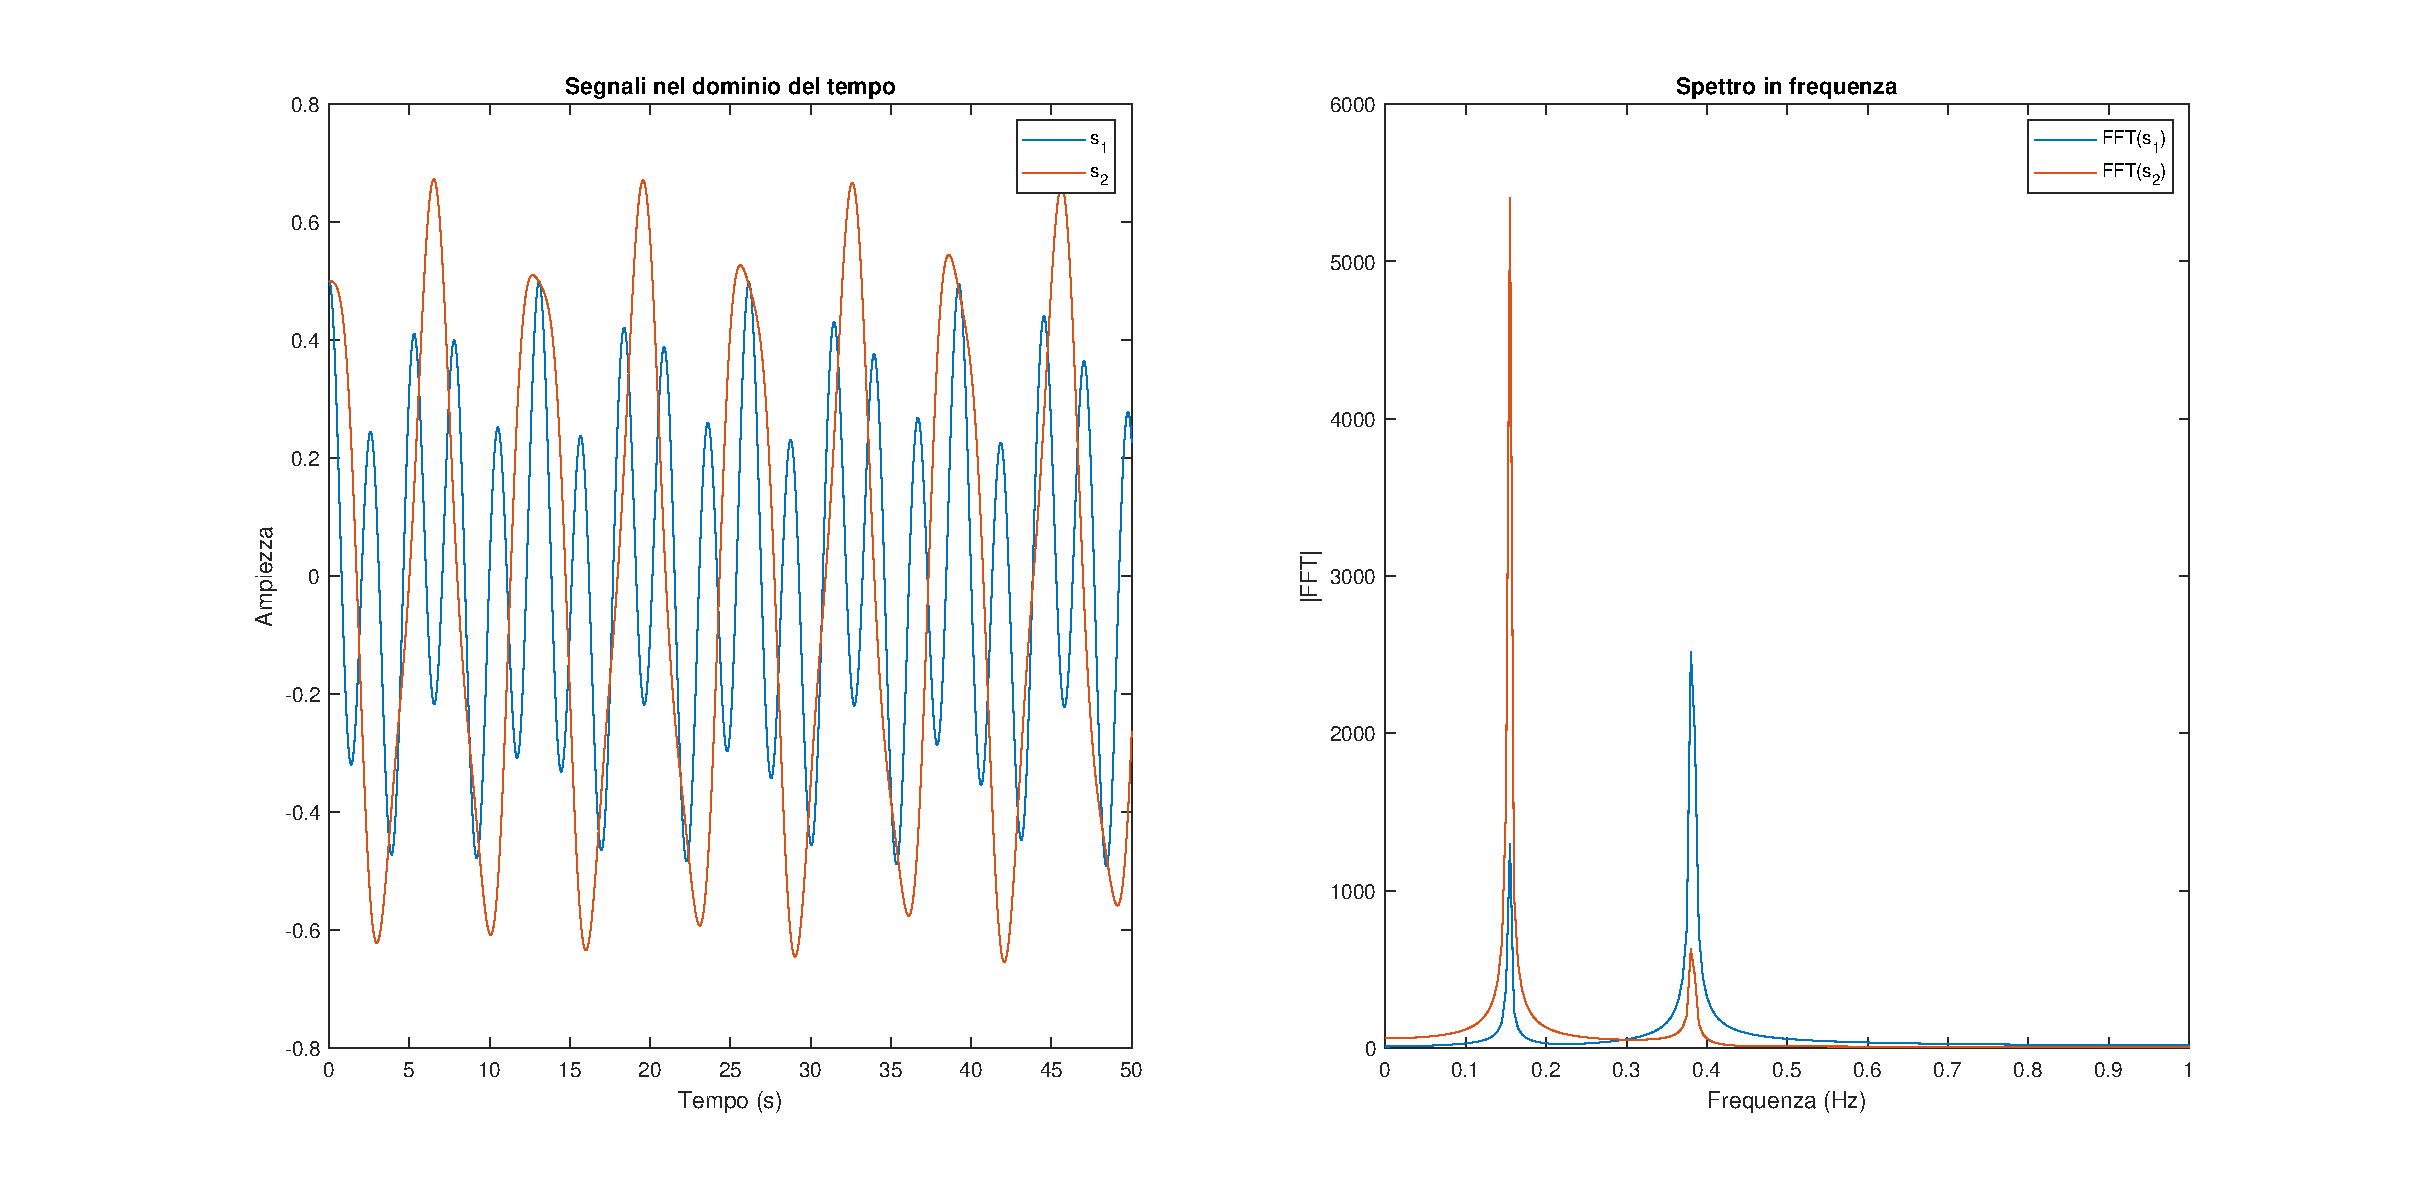
\includegraphics[scale=0.27]{media/1_Meccanica/spettro_segnali.eps}
\caption{Andamento delle soluzioni e relativa risposta spettrale}
\label{fig:1_spettro_segnali}
\end{figure}

Come si vede dalla trasformata di Fourier (\figurename~\ref{fig:1_spettro_segnali}), le soluzioni del sistema accoppiato contengono due frequenze di oscillazione ben distinte (\(\omega_{1}\) e \(\omega_{2}\)). A causa dell'interazione tra le due funzioni, entrambe le soluzioni \(y_{1}\) e \(y_{2}\) sono una combinazione di queste due frequenze, che sono differenti dal caso non interagente.
